\chapter{Моделирование}
\label{ch:chap3}


\section{Визуализация}

\begin{figure}[h]
\center{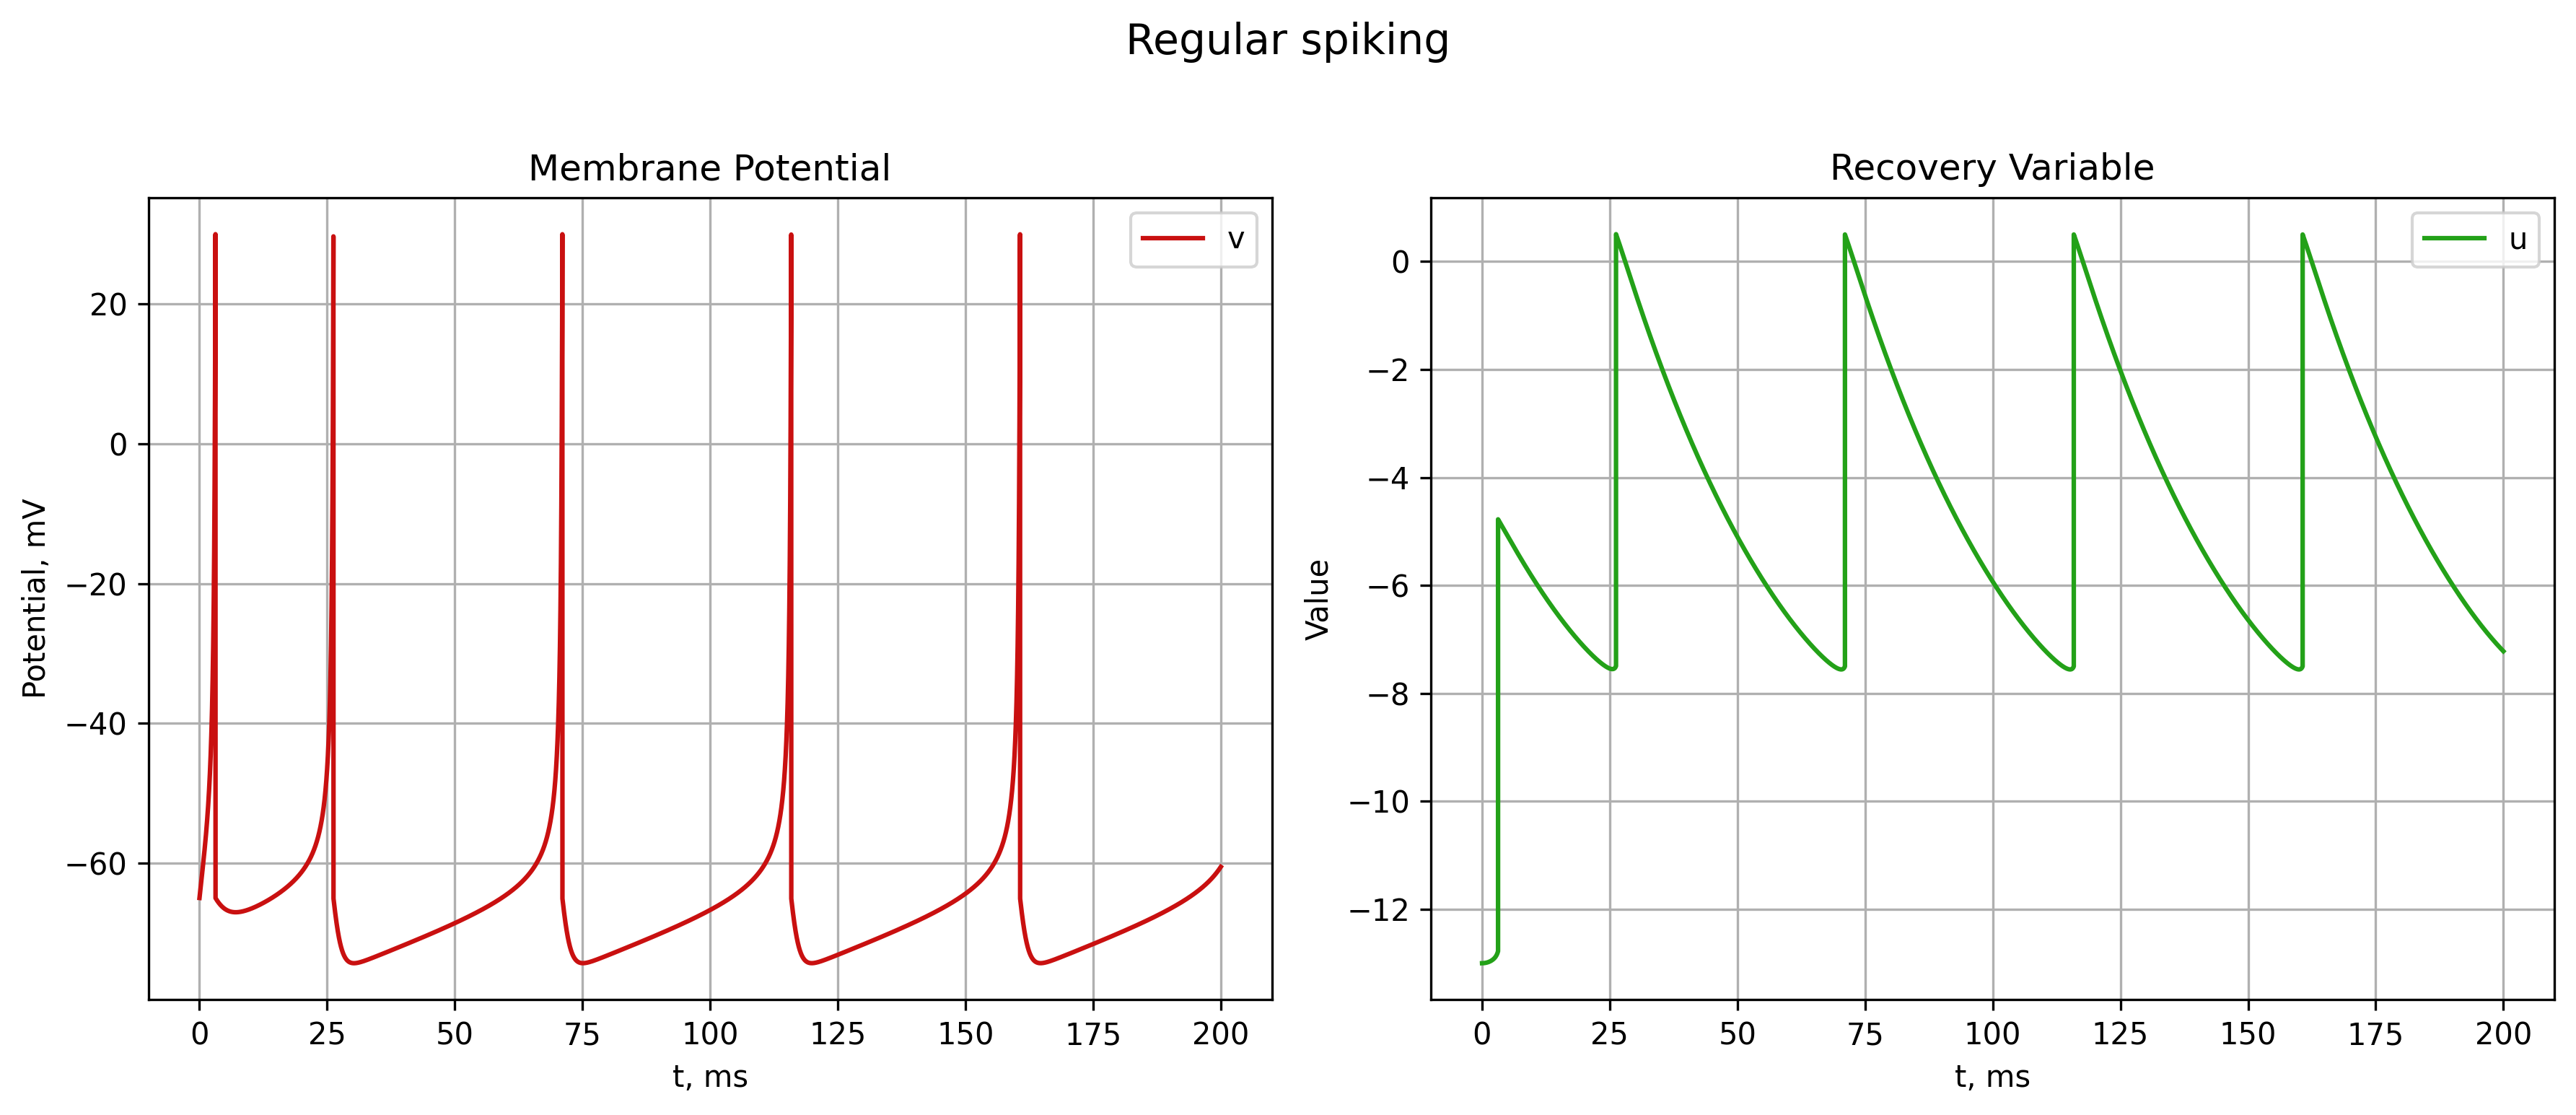
\includegraphics[width=1\linewidth]{pic/regular_spiking.png}}
\caption{Визуализация регулярно-спайкового нейрона при $I=10$ нА.}
\label{1_rs}
\end{figure}

\begin{figure}[h]
	\center{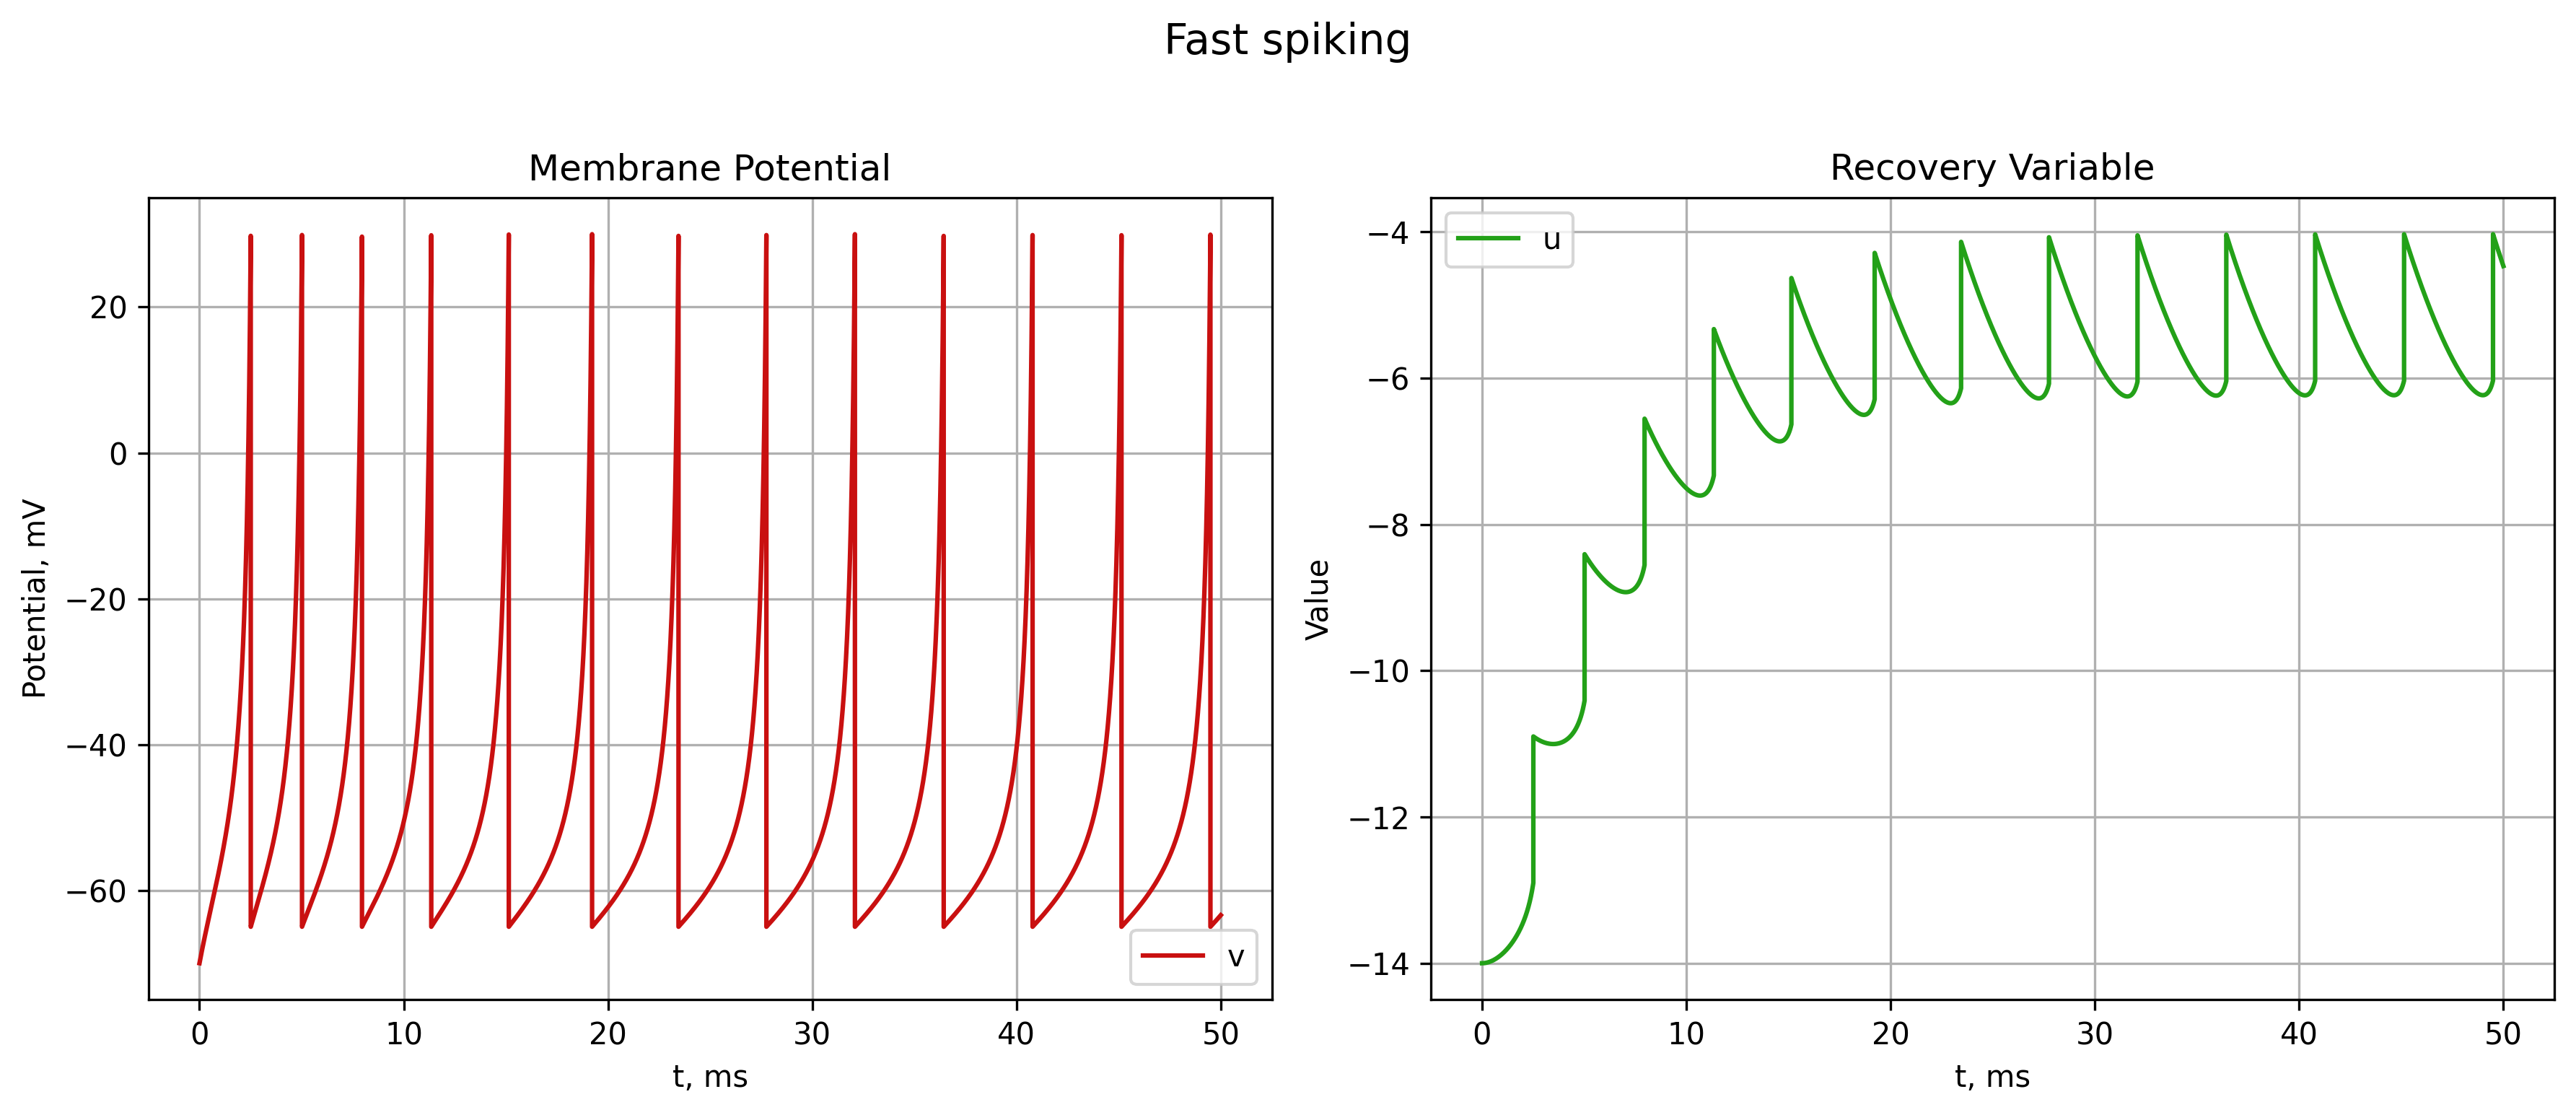
\includegraphics[width=1\linewidth]{pic/fast_spiking.png}}
	\caption{Визуализация быстро-спайкового нейрона при $I=15$ нА.}
	\label{1_fs}
\end{figure}

\begin{figure}[h]
	\center{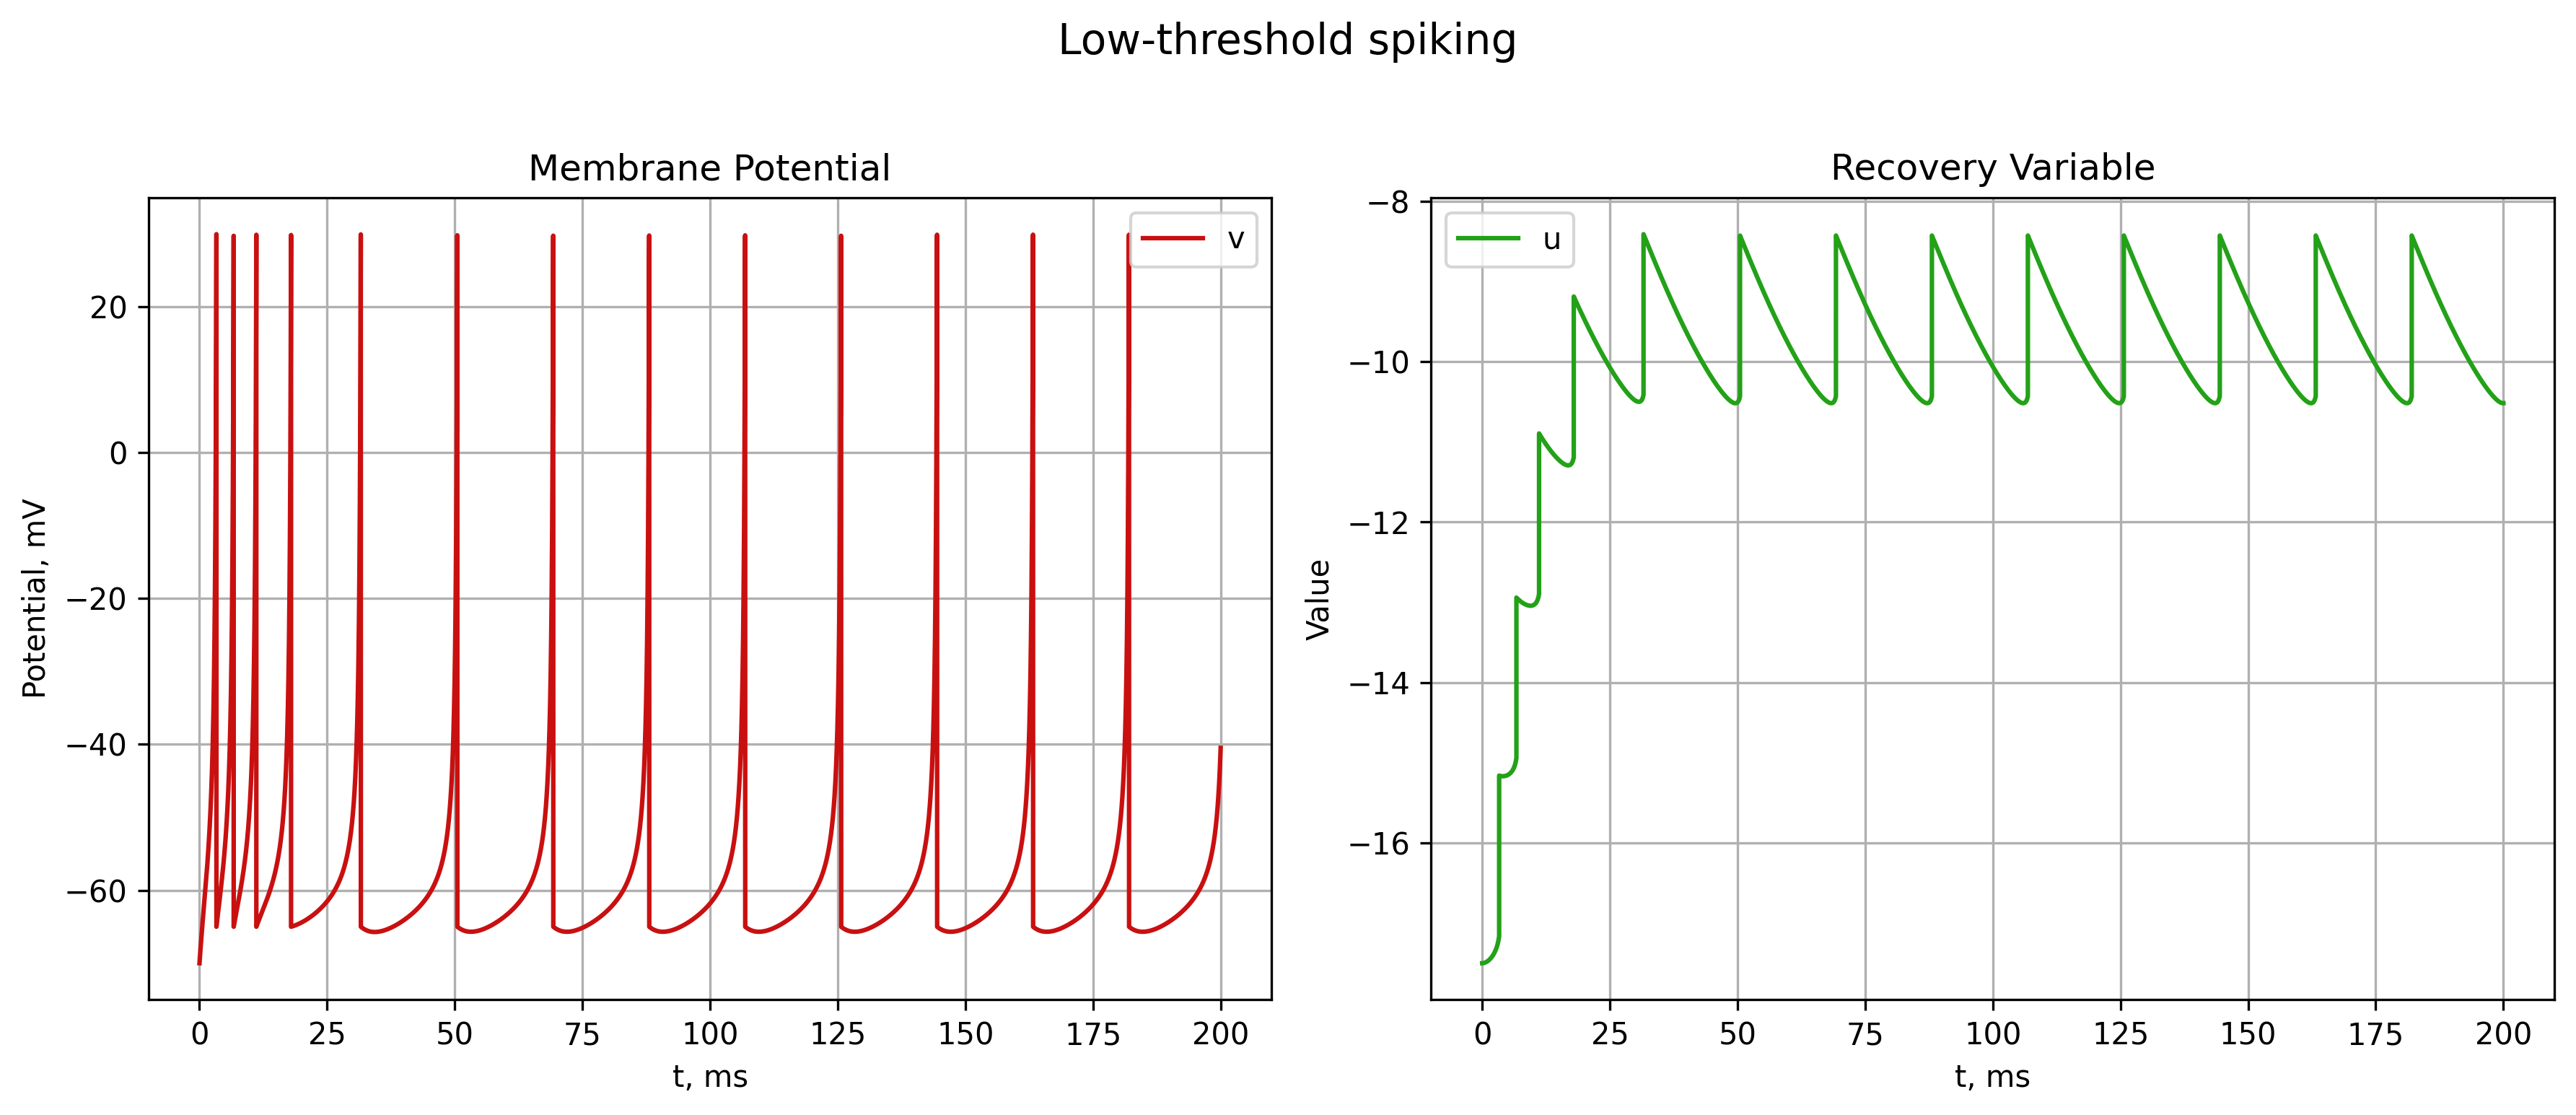
\includegraphics[width=1\linewidth]{pic/low_threshold_spiking.png}}
	\caption{Визуализация низкопорогового спайкового нейрона при $I=7$ нА.}
	\label{1_lts}
\end{figure}

\begin{figure}[h]
	\center{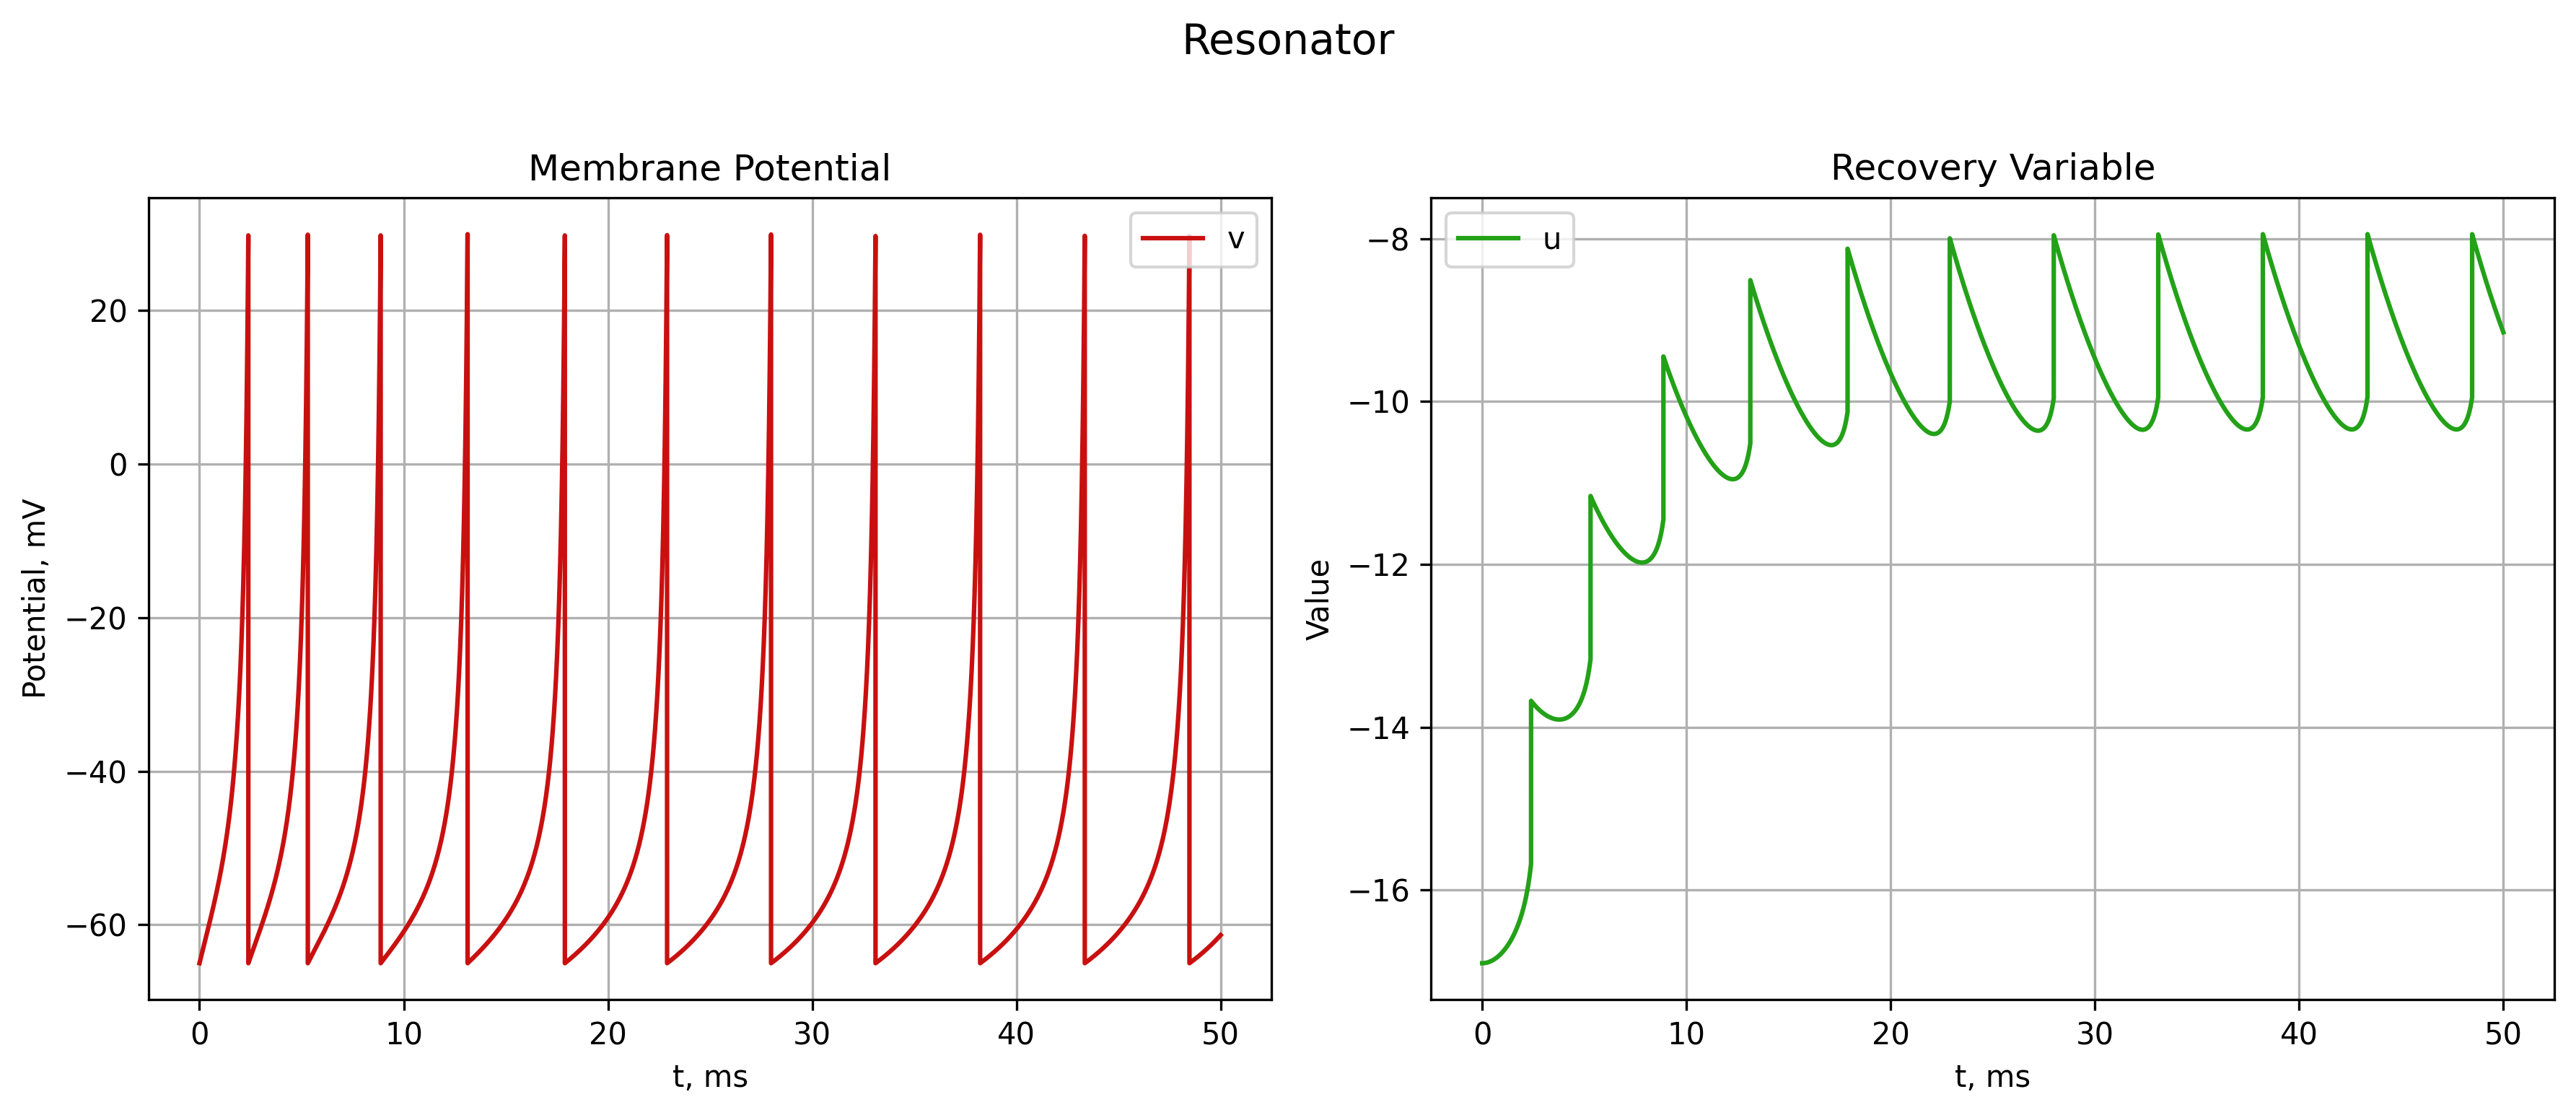
\includegraphics[width=1\linewidth]{pic/resonator_spiking.png}}
	\caption{Визуализация резонансного нейрона при $I=10$ нА.}
	\label{1_rz}
\end{figure}

\begin{figure}[h]
	\center{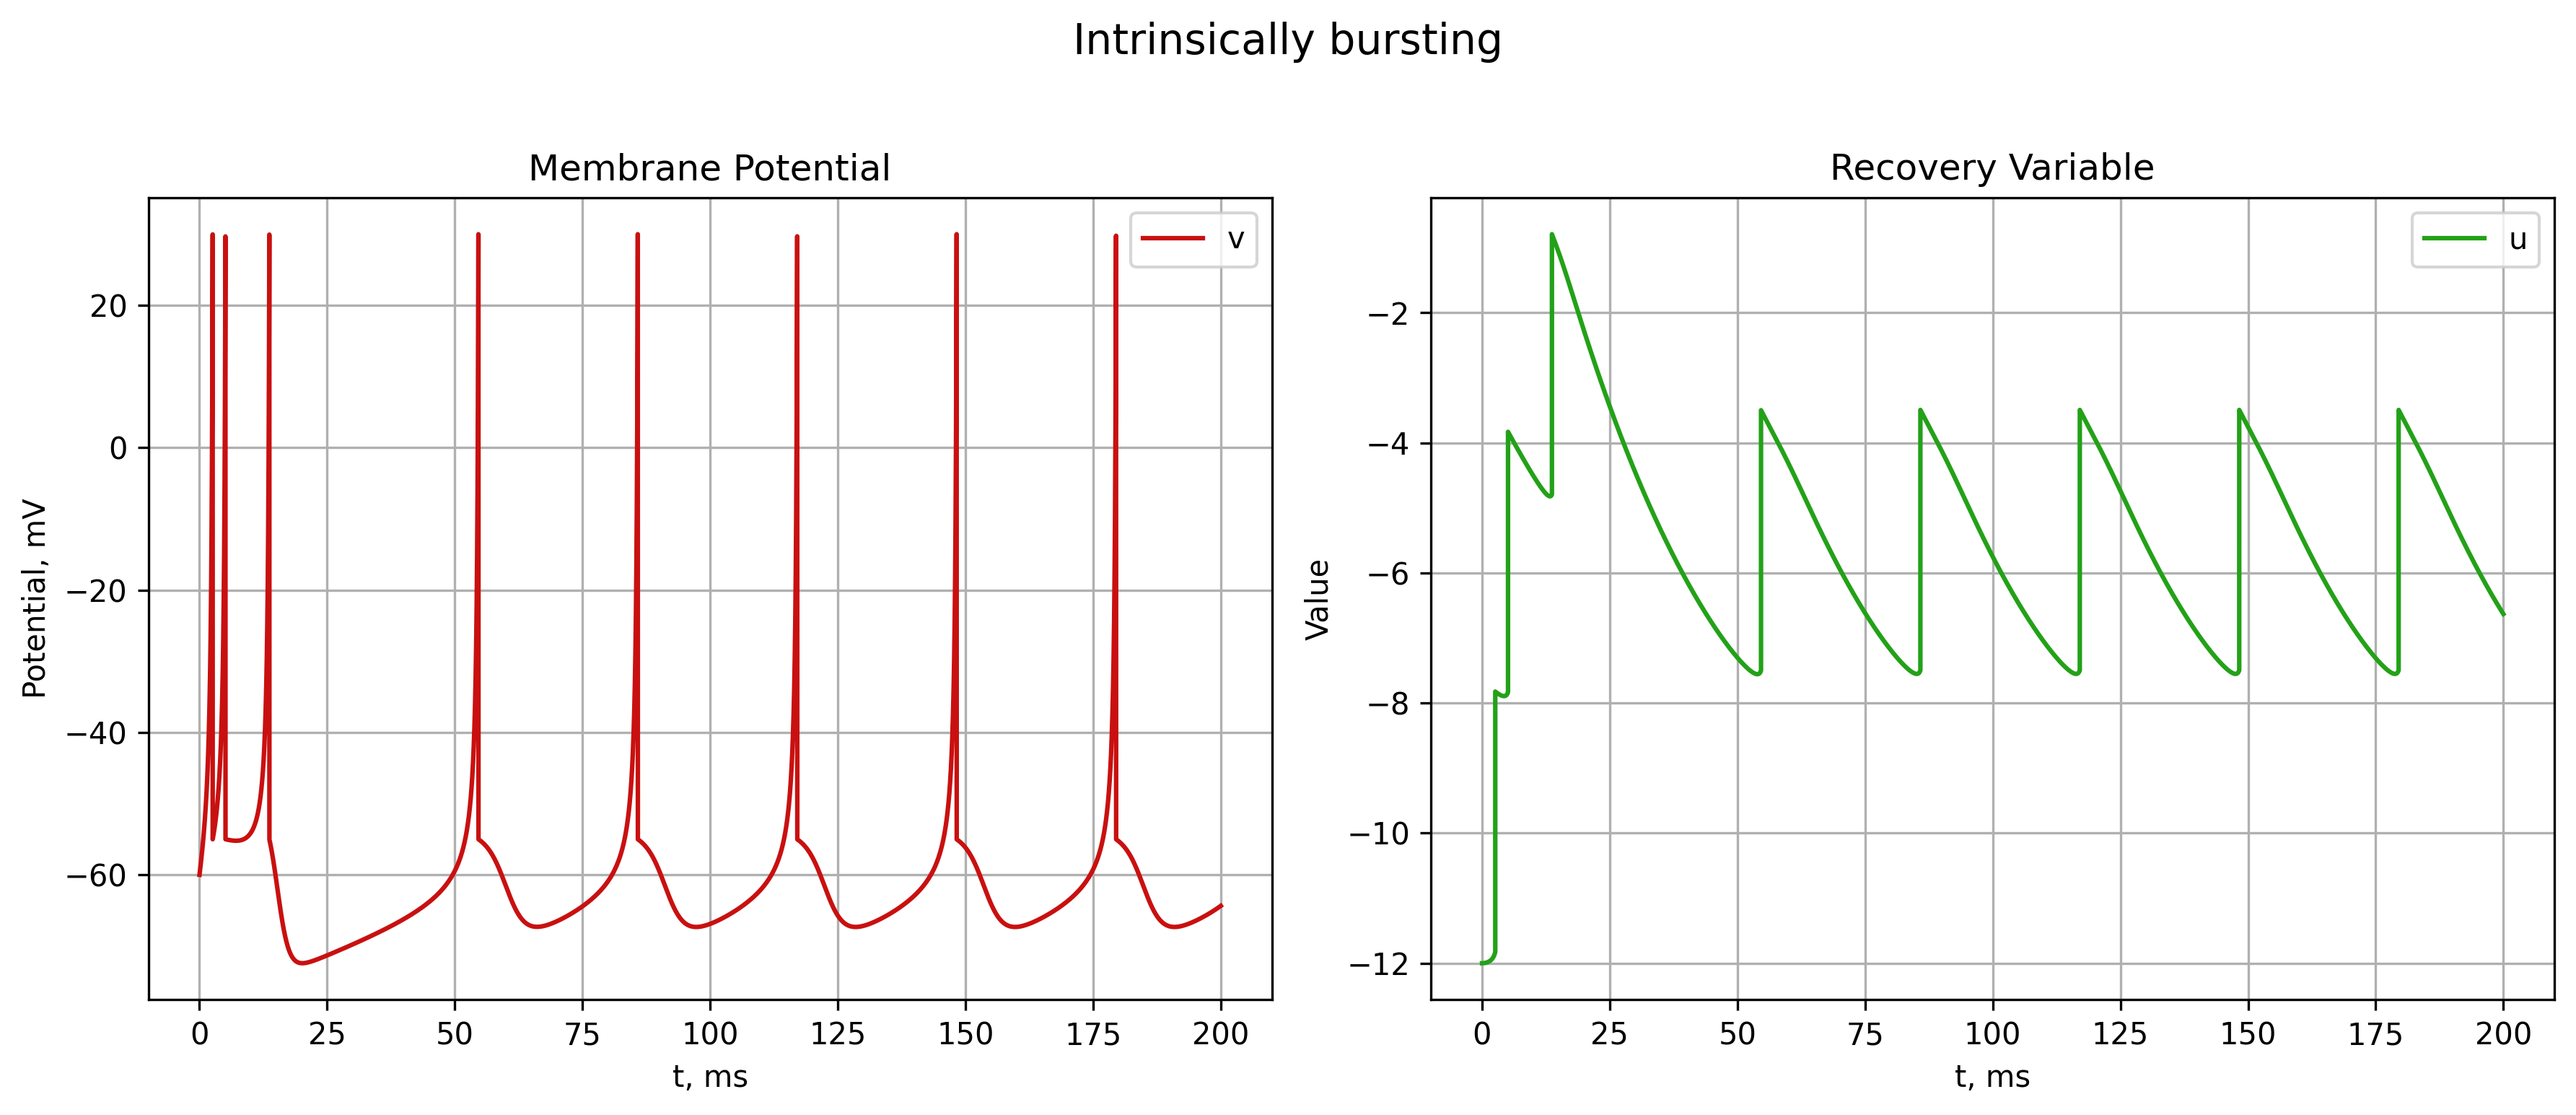
\includegraphics[width=1\linewidth]{pic/intrinsically_bursting.png}}
	\caption{Визуализация внутренне разрывного нейрона при $I=10$ нА.}
	\label{1_ib}
\end{figure}

\begin{figure}[h]
	\center{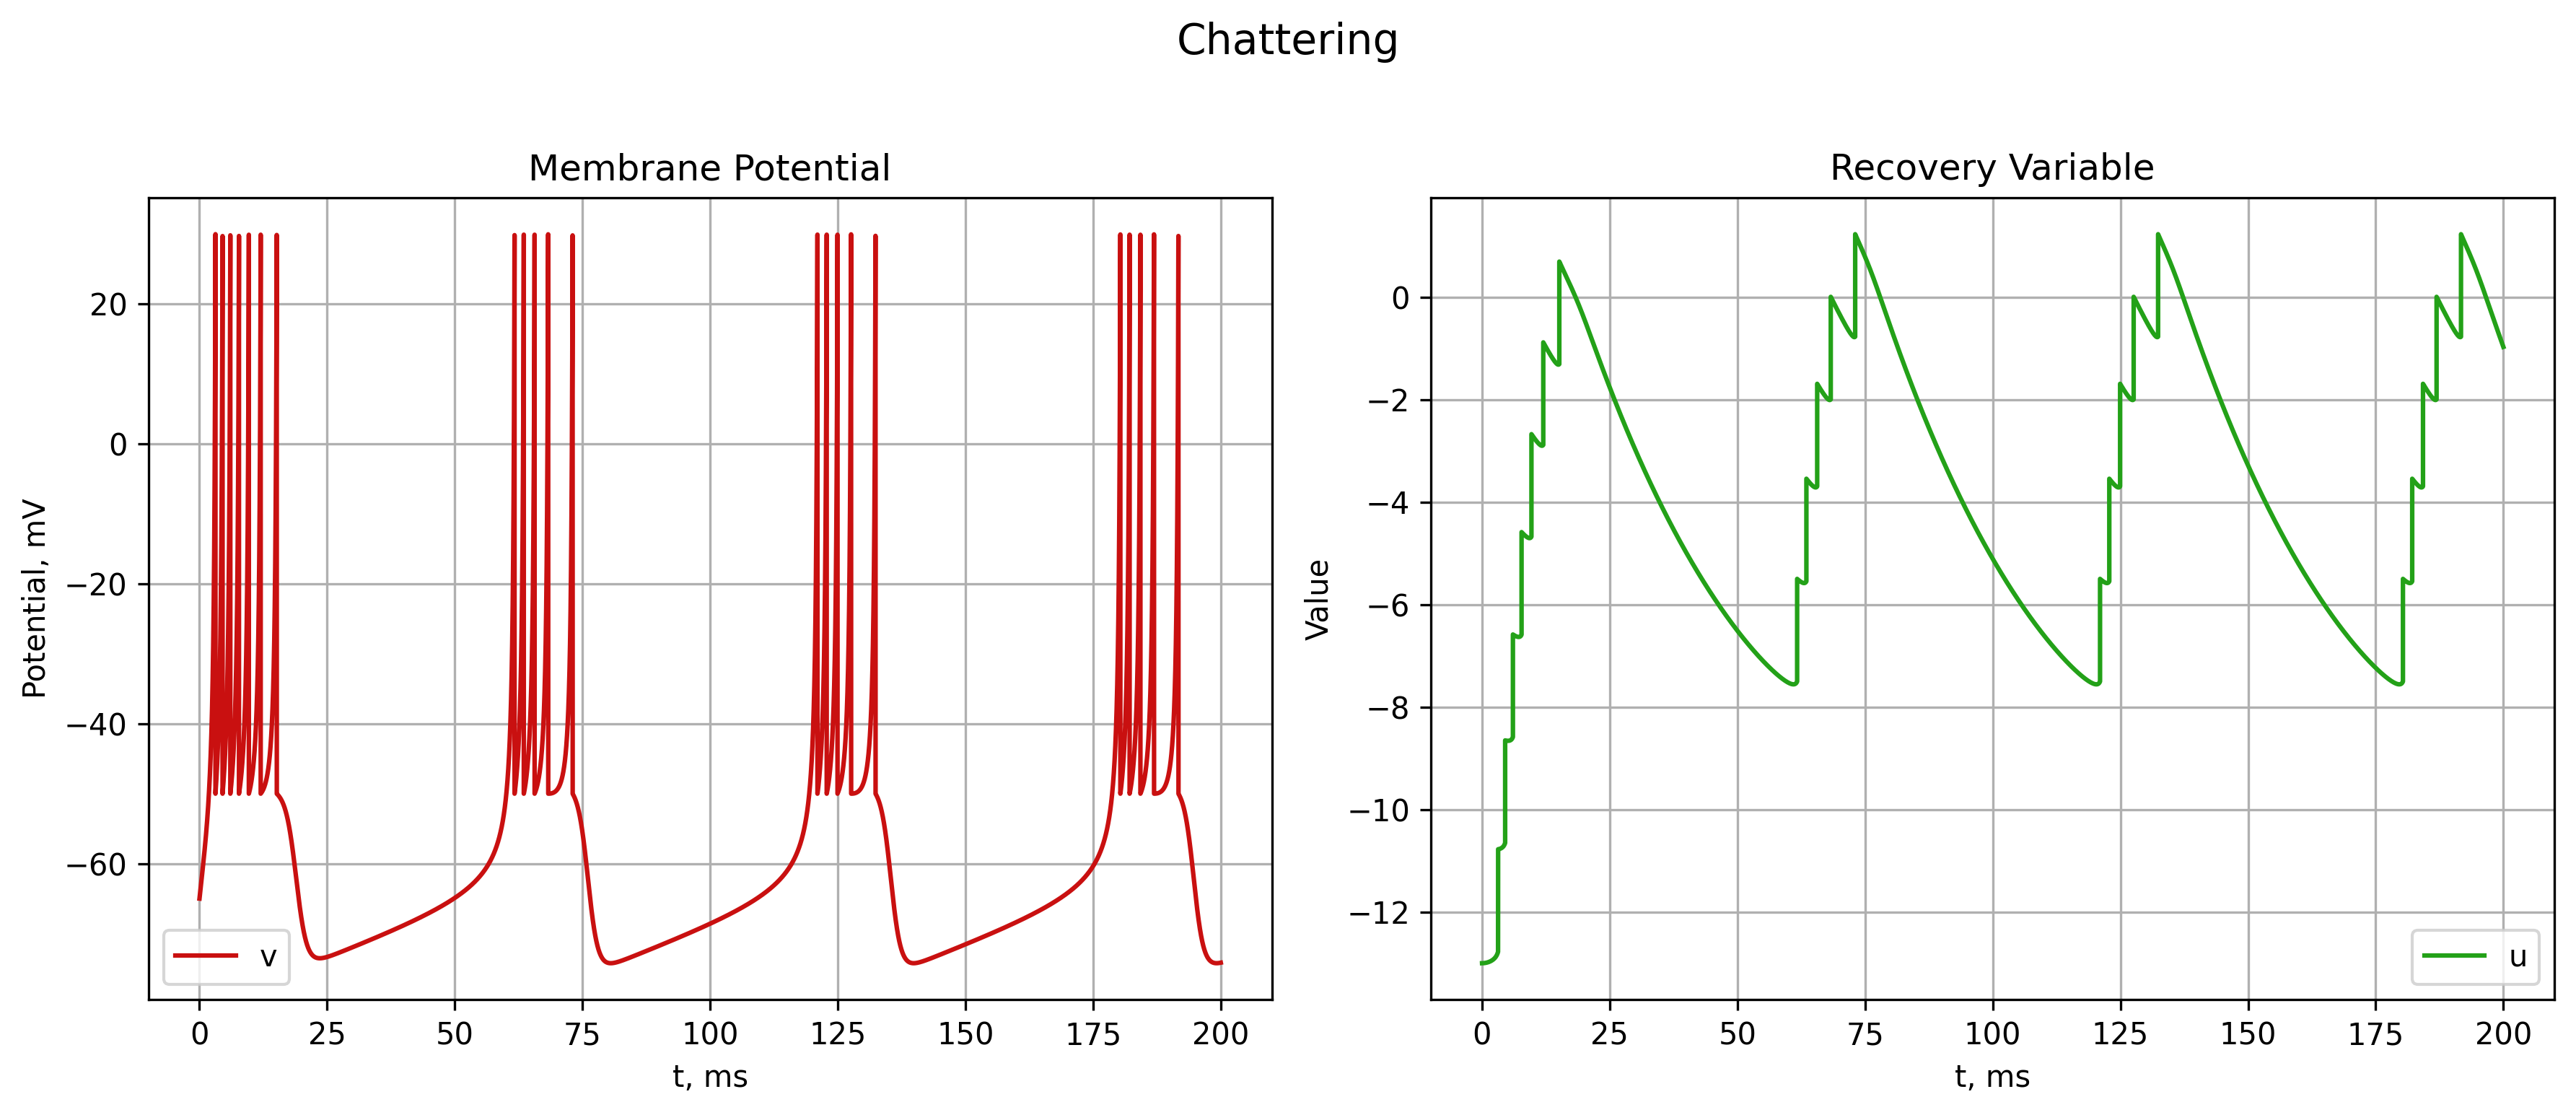
\includegraphics[width=1\linewidth]{pic/chattering.png}}
	\caption{Визуализация чаттерного нейрона при $I=10$ нА.}
	\label{1_ch}
\end{figure}

\begin{figure}[h]
	\center{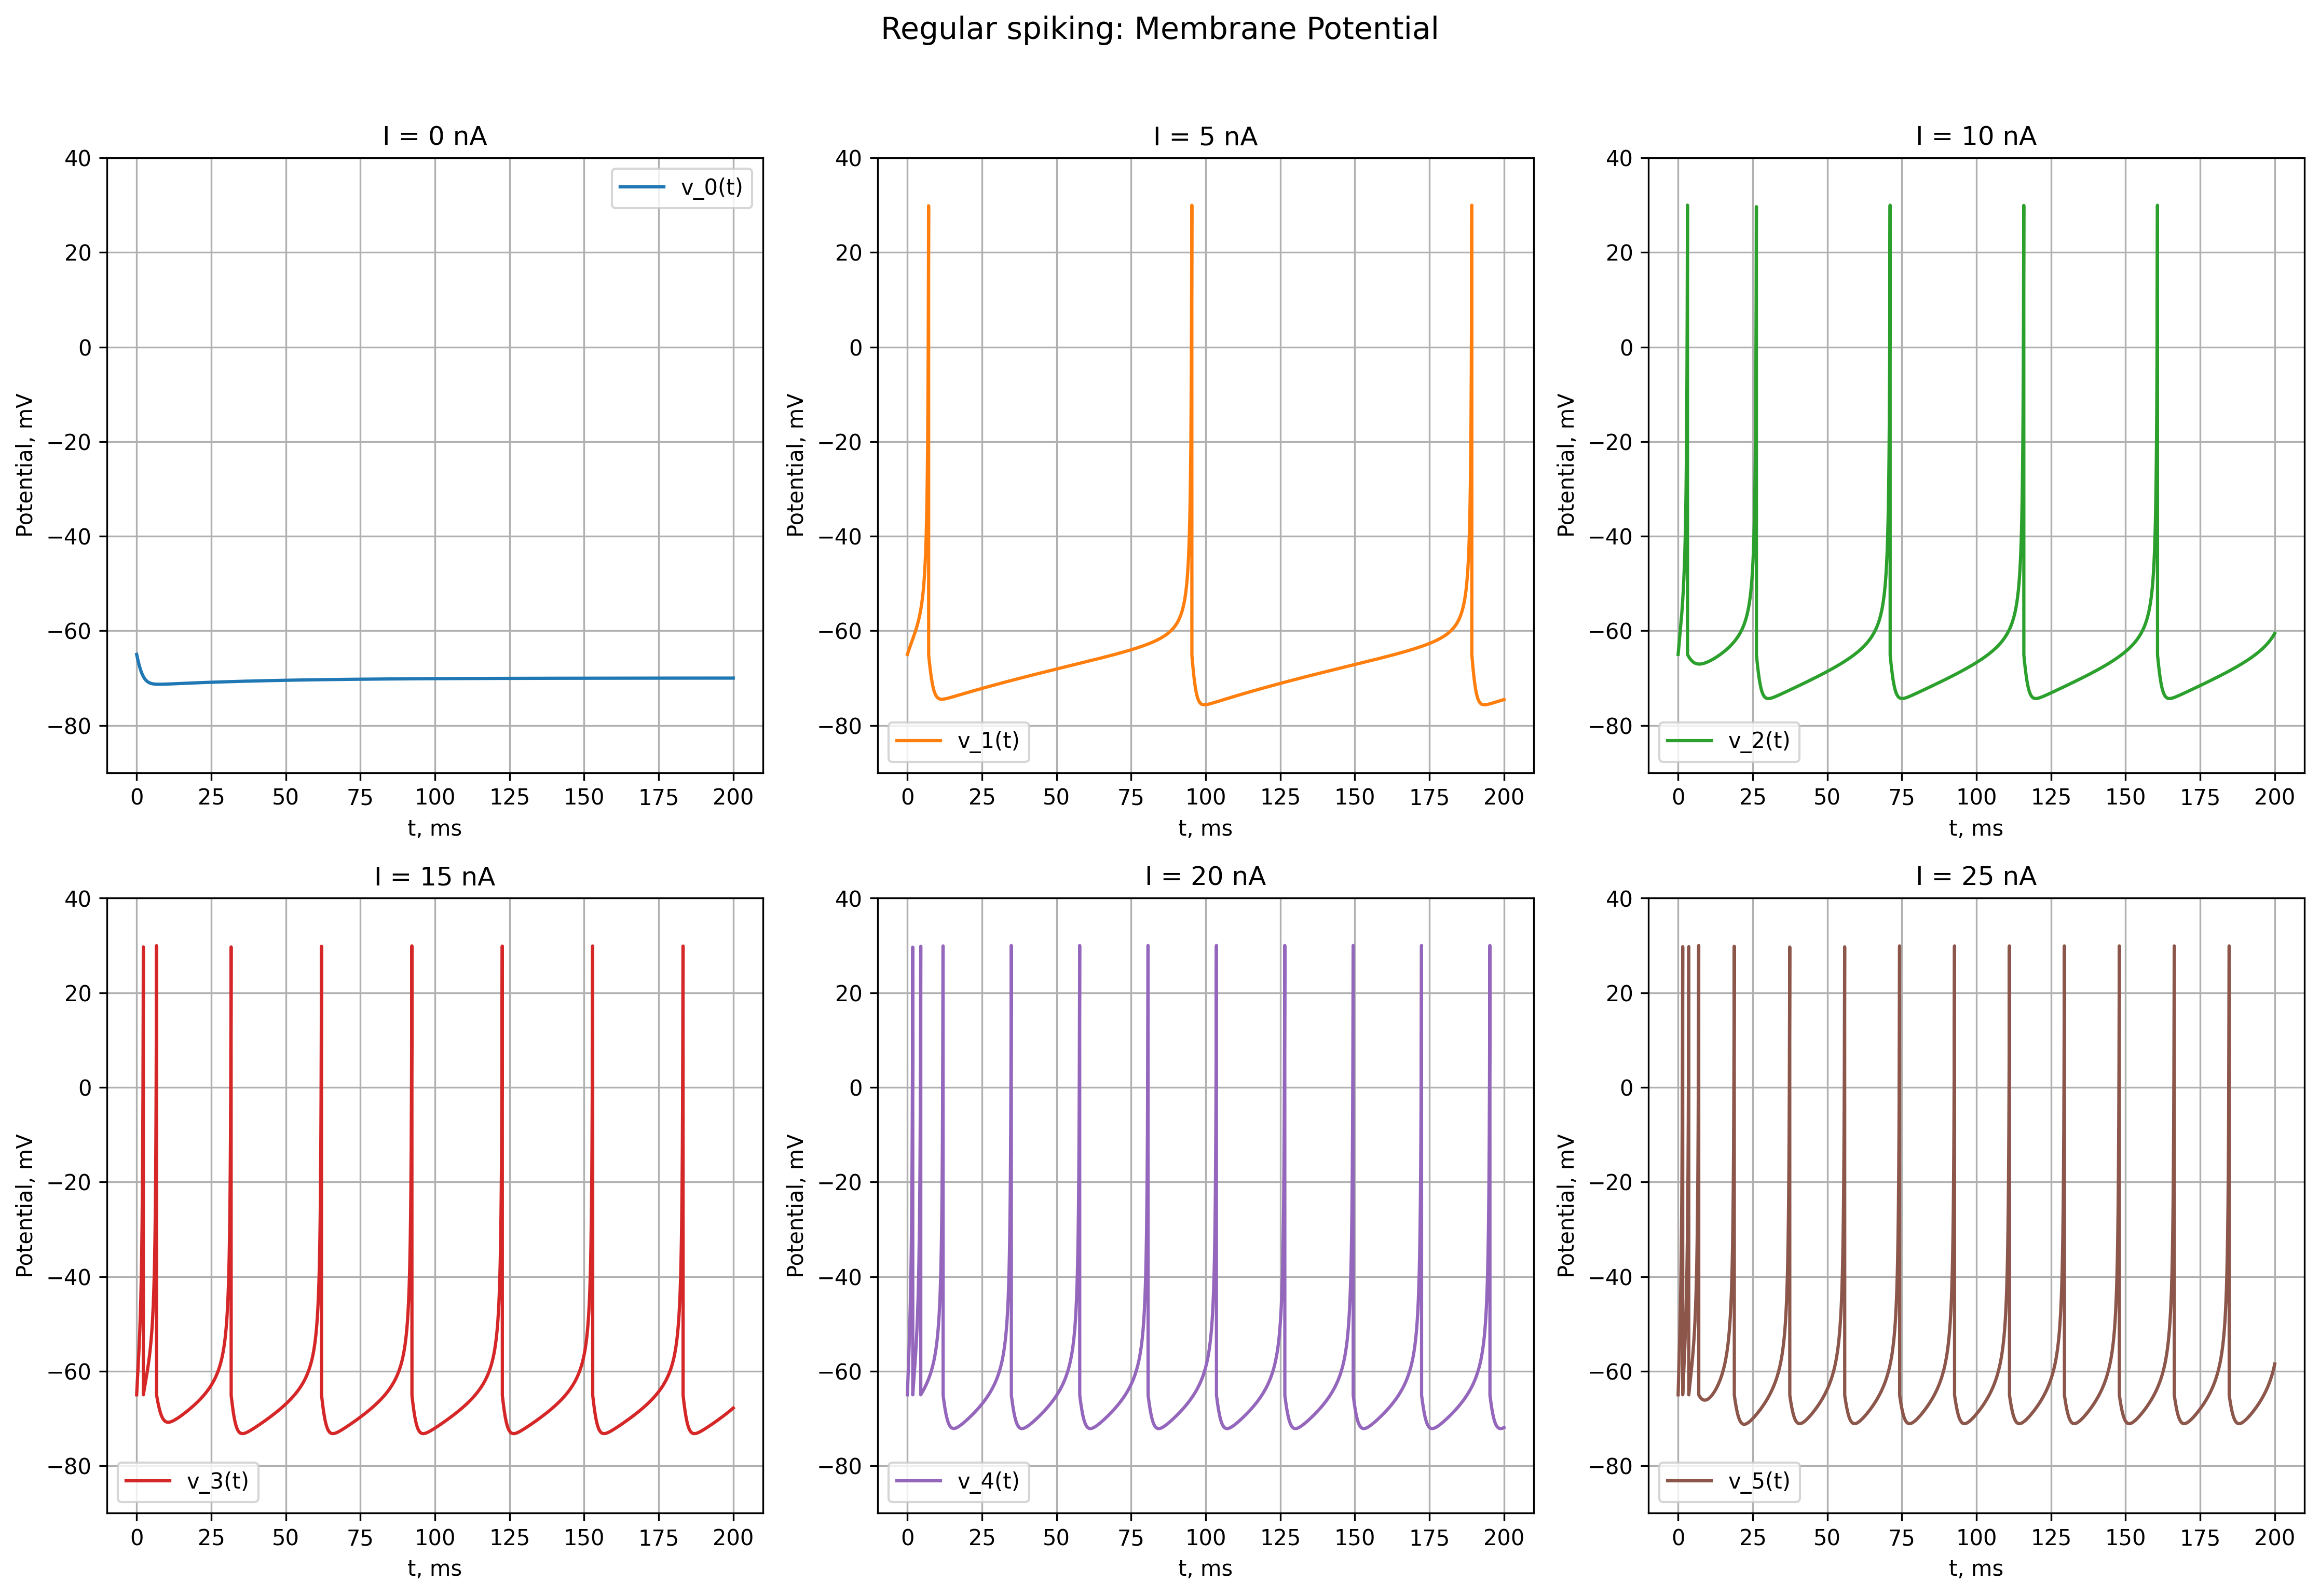
\includegraphics[width=1\linewidth]{pic/rs_different_I_potentials.png}}
	\caption{Графики $v(t)$ регулярно-спайкового нейрона для разных значений $I$.}
	\label{rs_different_I_potentials}
\end{figure}

\begin{figure}[h]
	\center{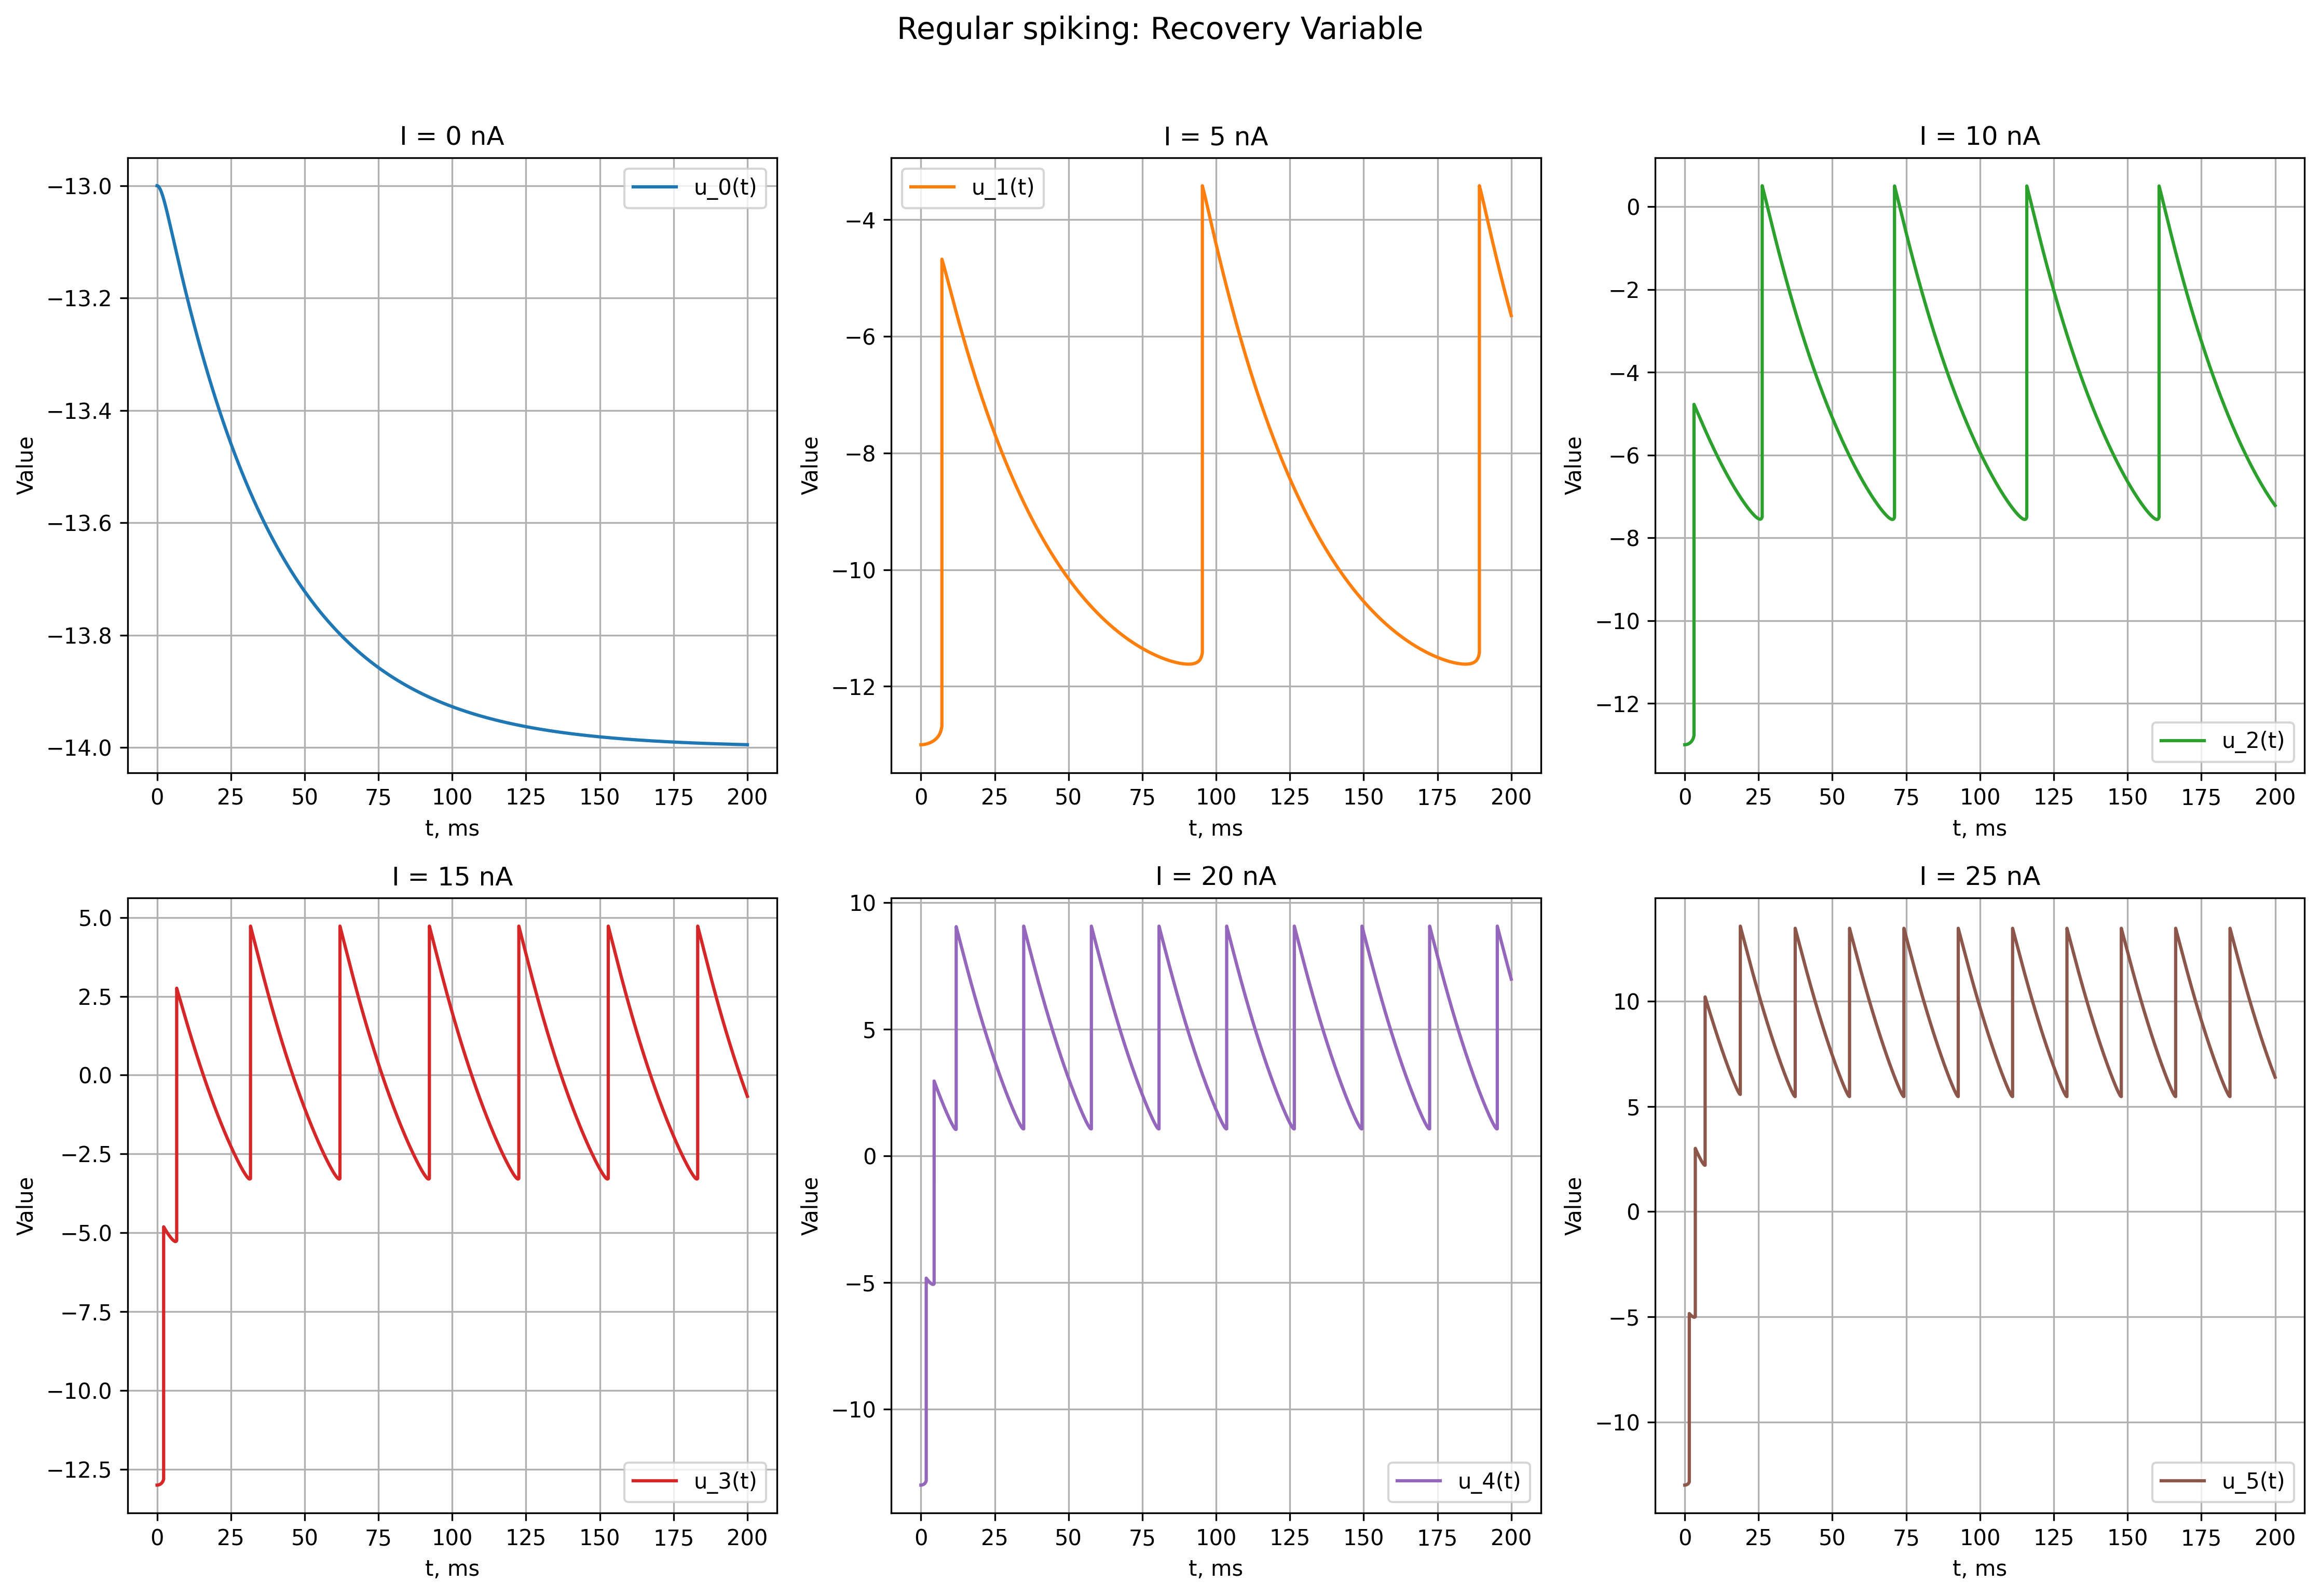
\includegraphics[width=1\linewidth]{pic/rs_different_I_recovery.png}}
	\caption{Графики $u(t)$ регулярно-спайкового нейрона для разных значений $I$.}
	\label{rs_different_I_recovery}
\end{figure}

\begin{figure}[h]
	\center{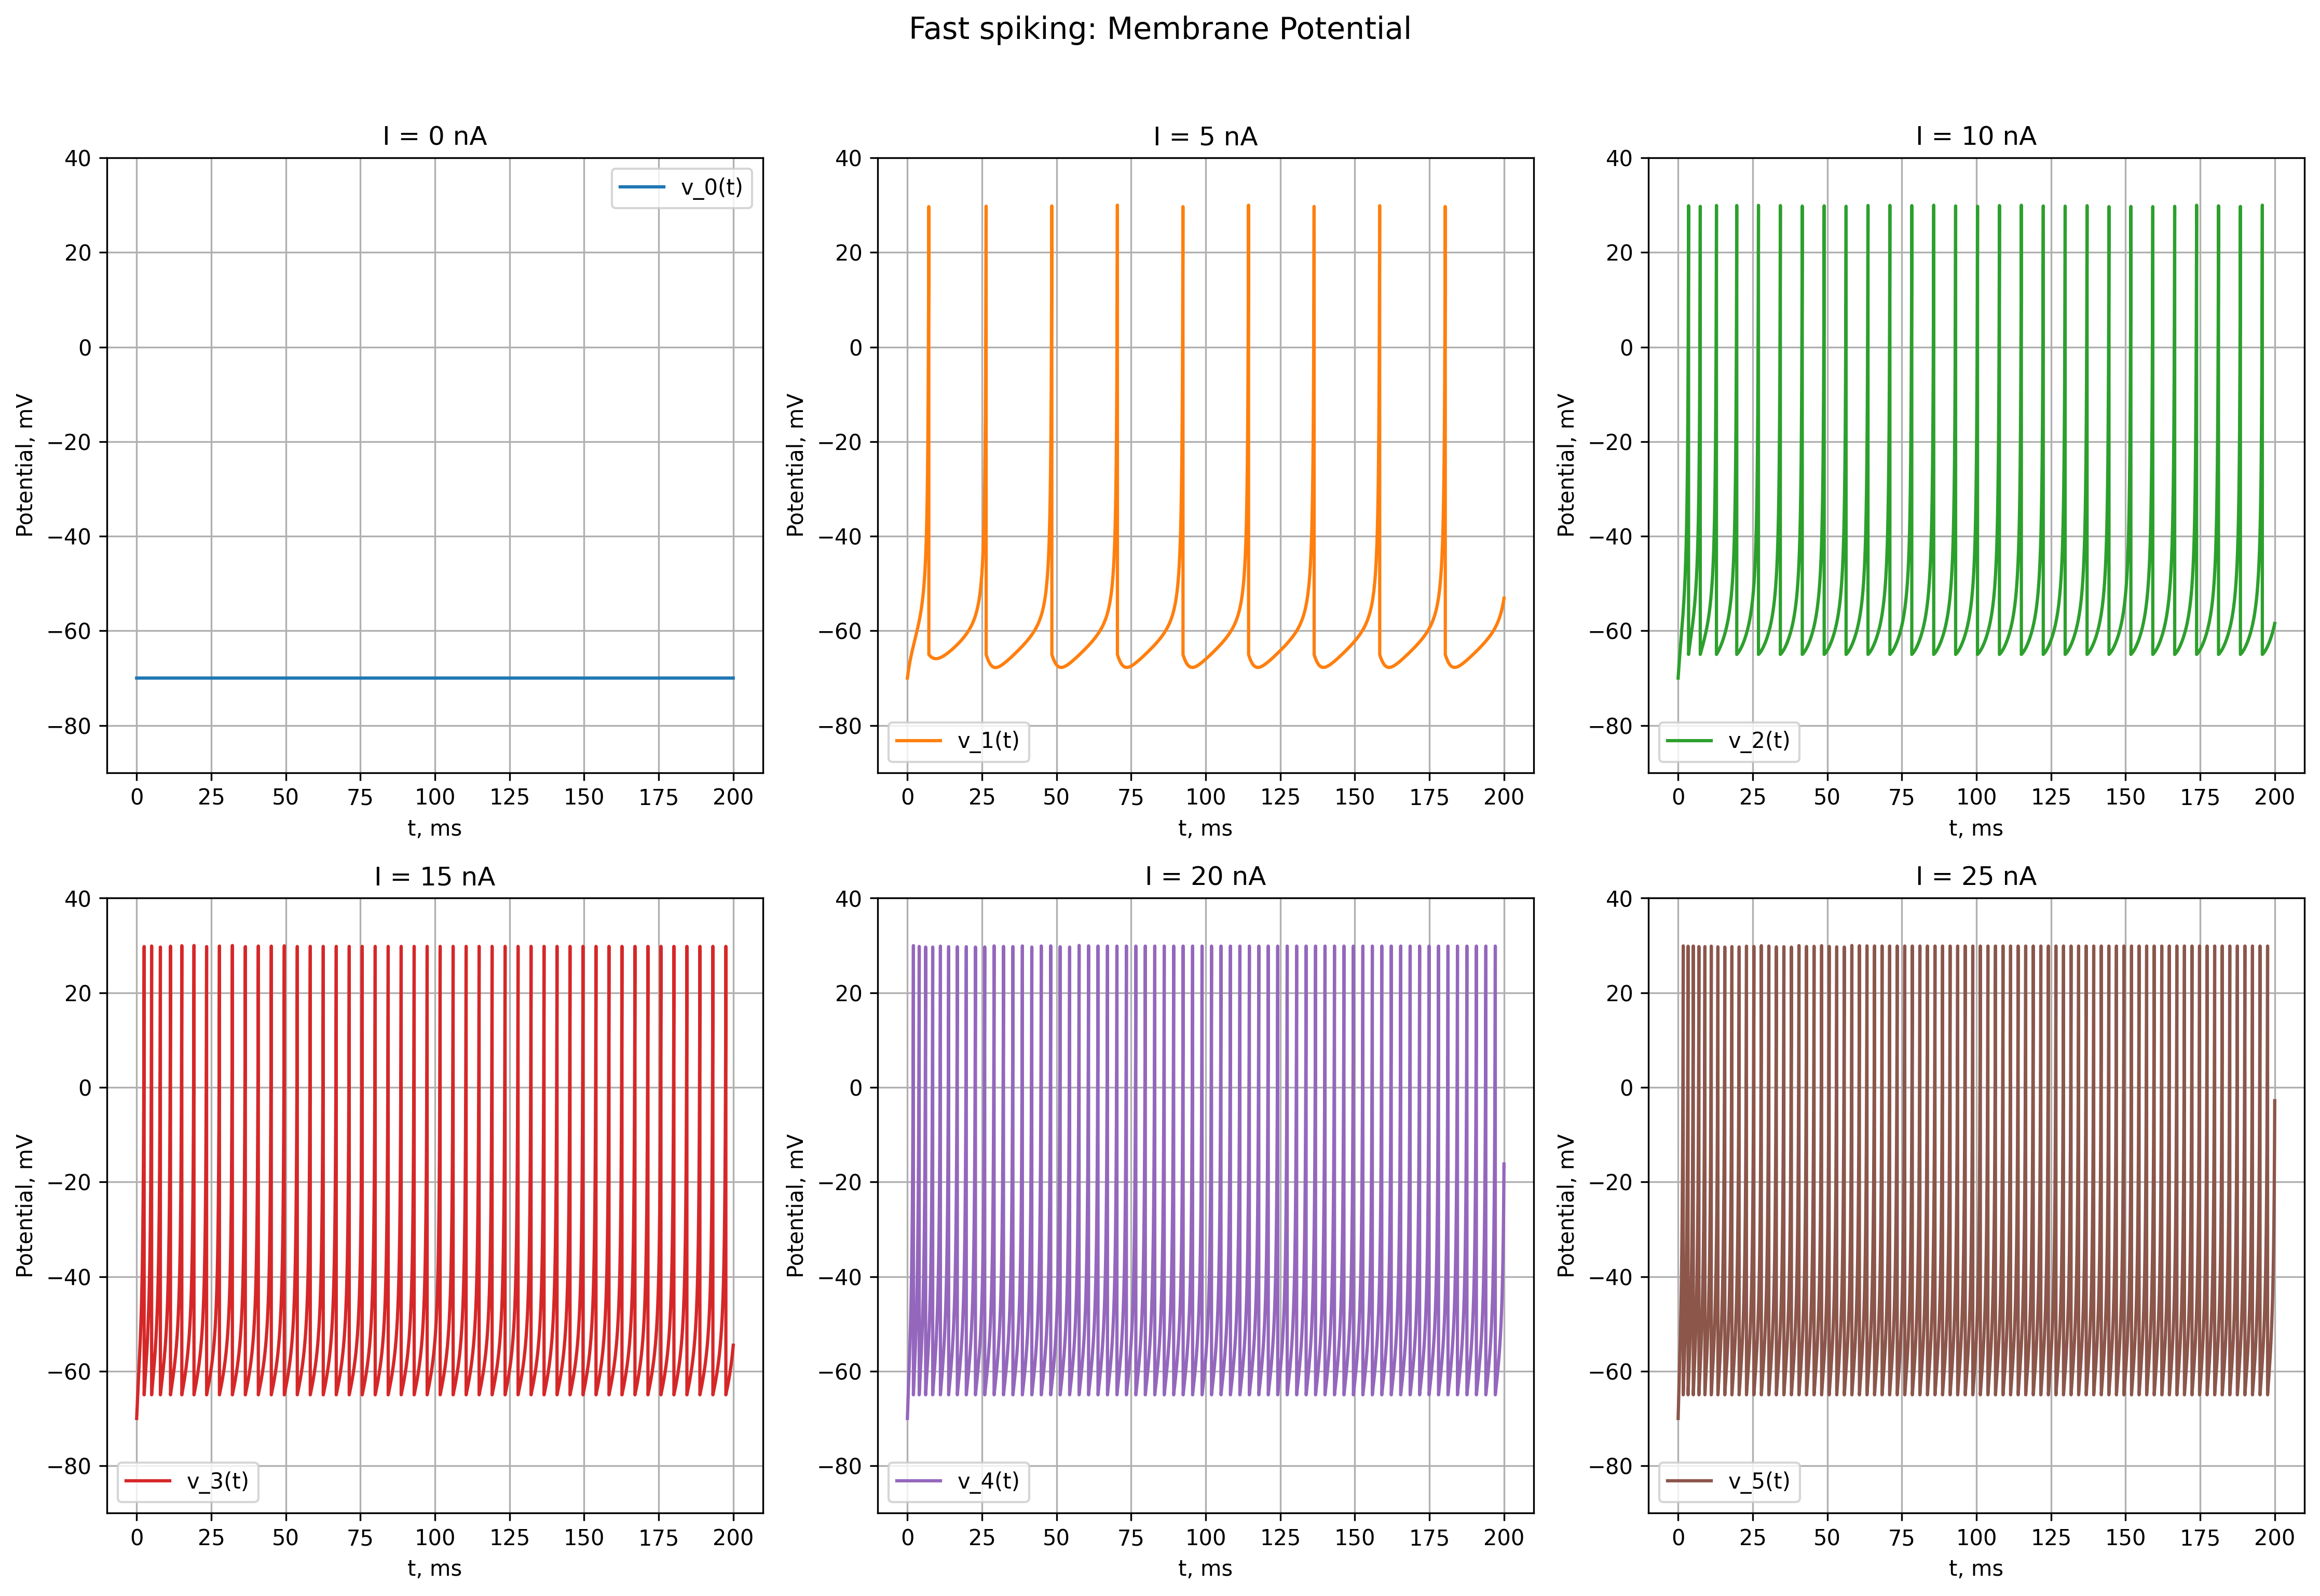
\includegraphics[width=1\linewidth]{pic/fs_different_I_potentials.png}}
	\caption{Графики $v(t)$ быстро-спайкового нейрона для разных значений $I$.}
	\label{fs_different_I_potentials}
\end{figure}

\begin{figure}[h]
	\center{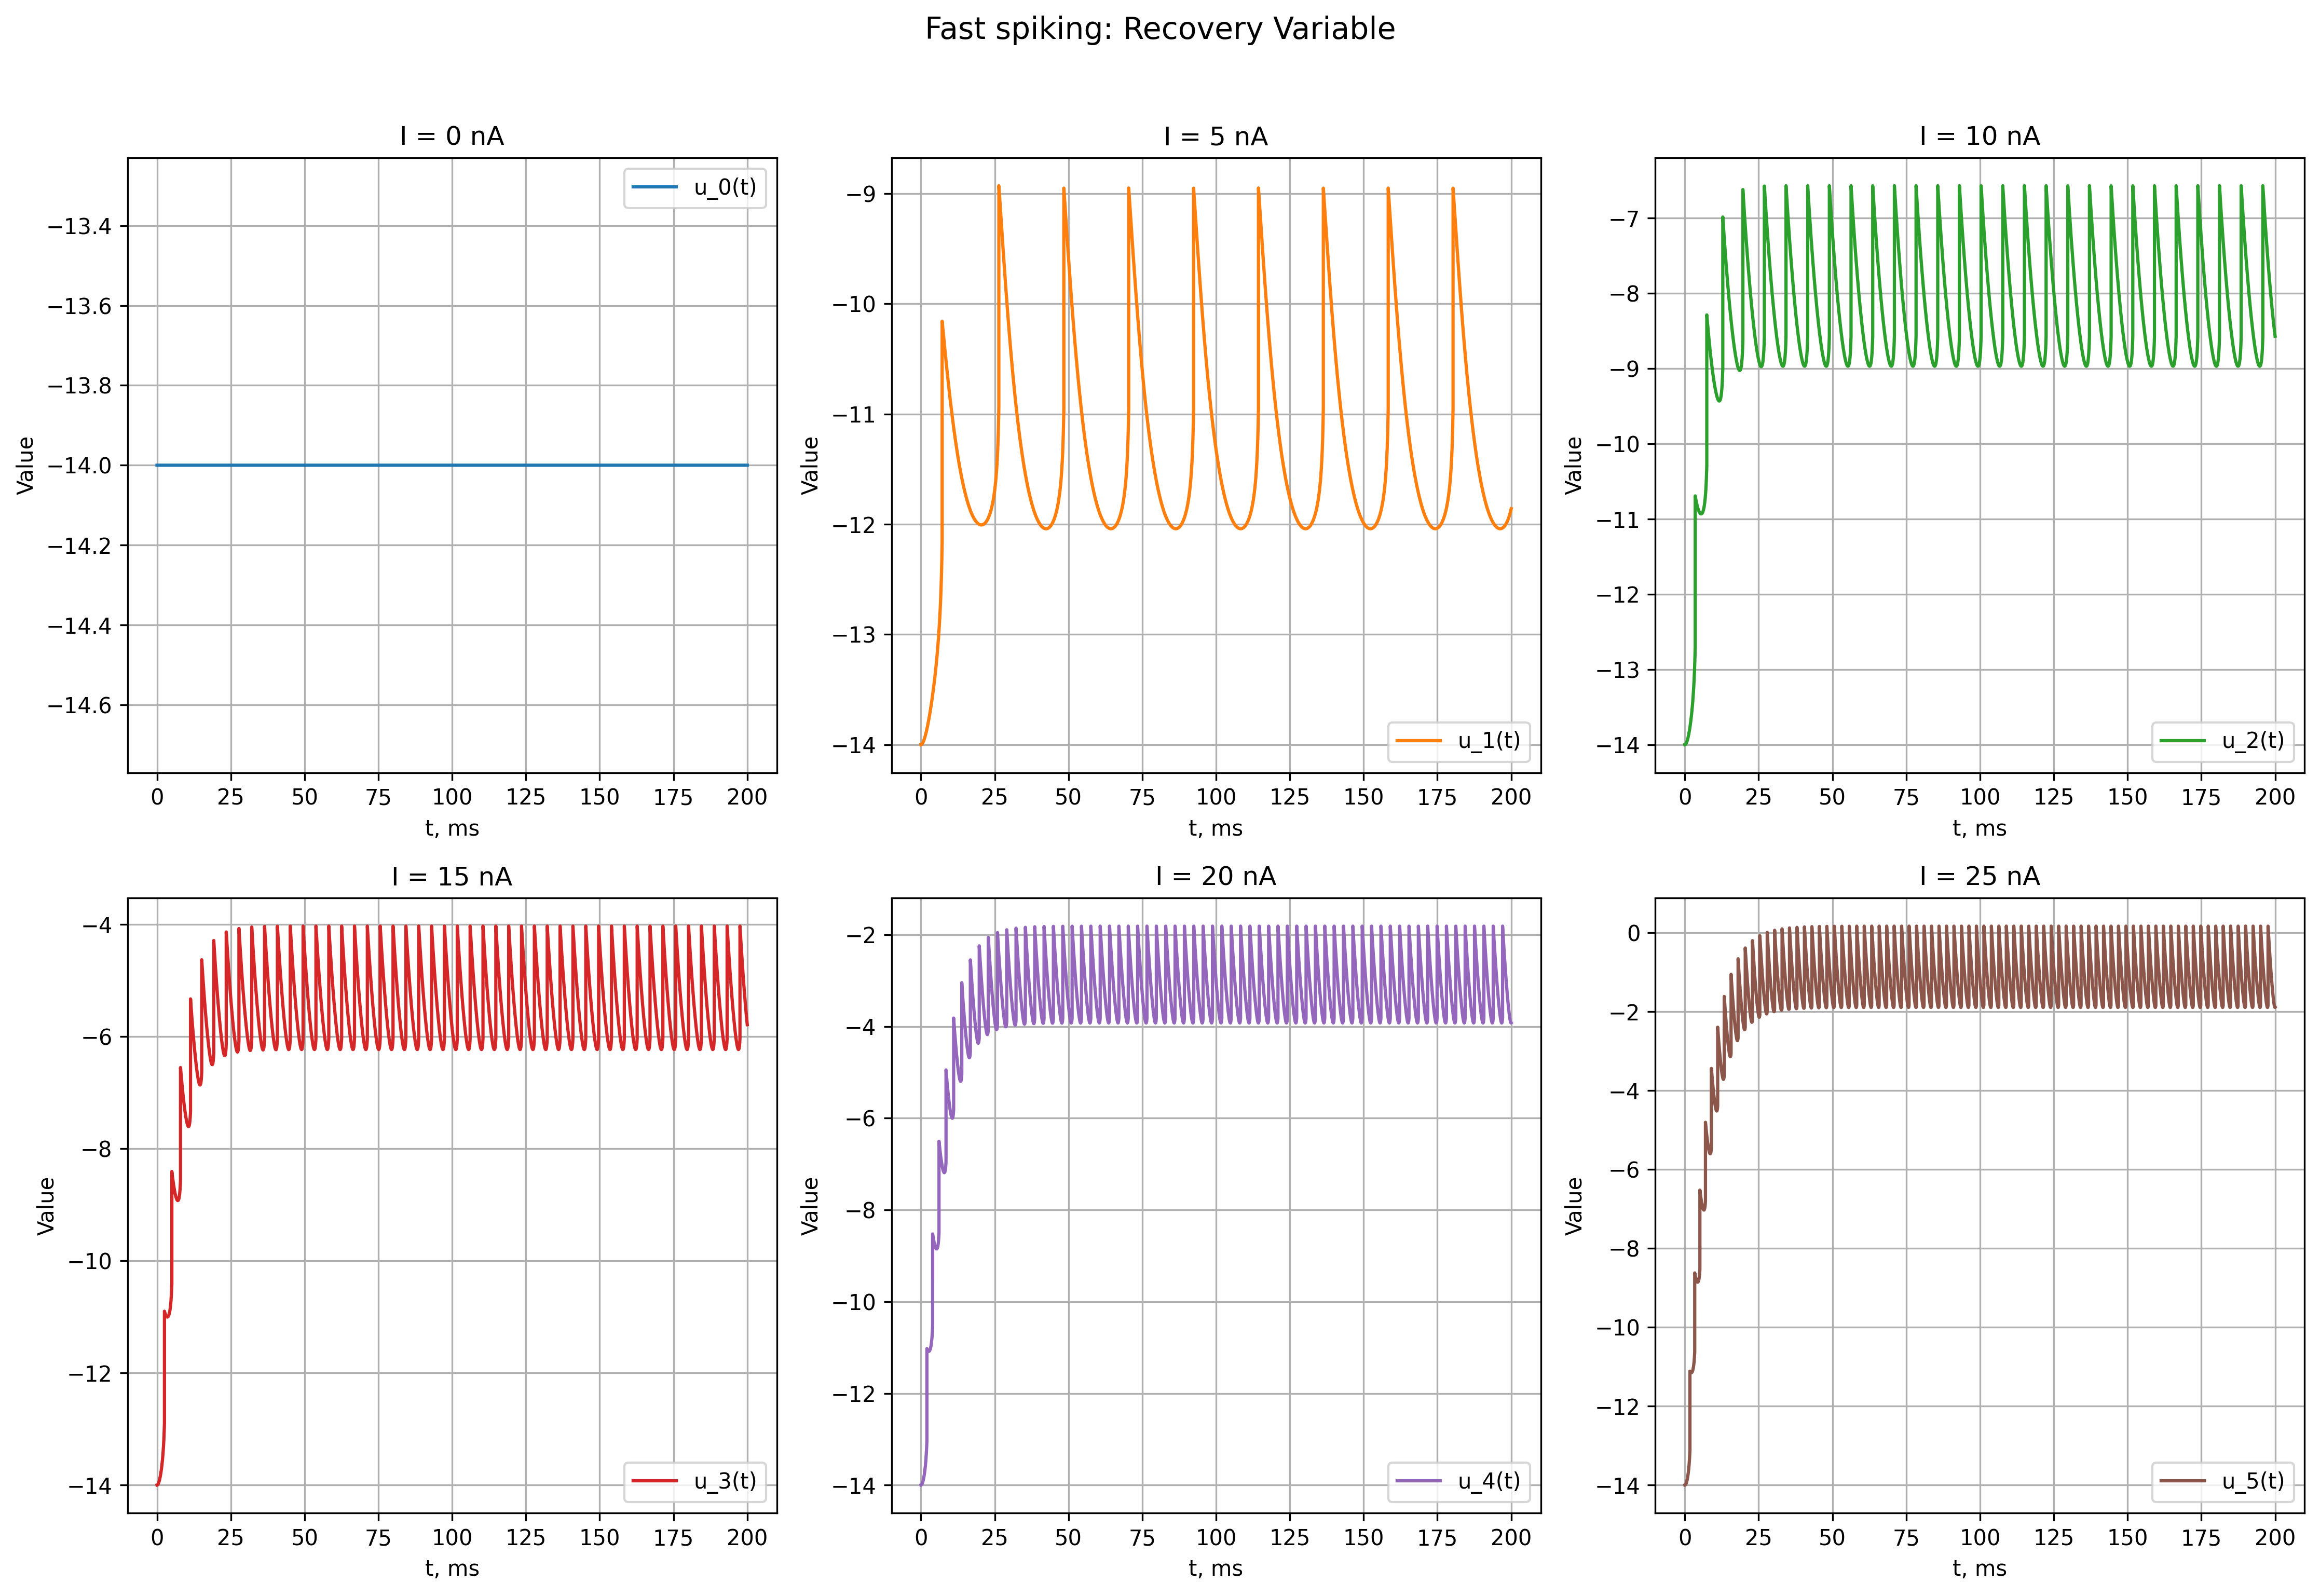
\includegraphics[width=1\linewidth]{pic/fs_different_I_recovery.png}}
	\caption{Графики $u(t)$ быстро-спайкового нейрона для разных значений $I$.}
	\label{fs_different_I_recovery}
\end{figure}

\begin{figure}[h]
	\center{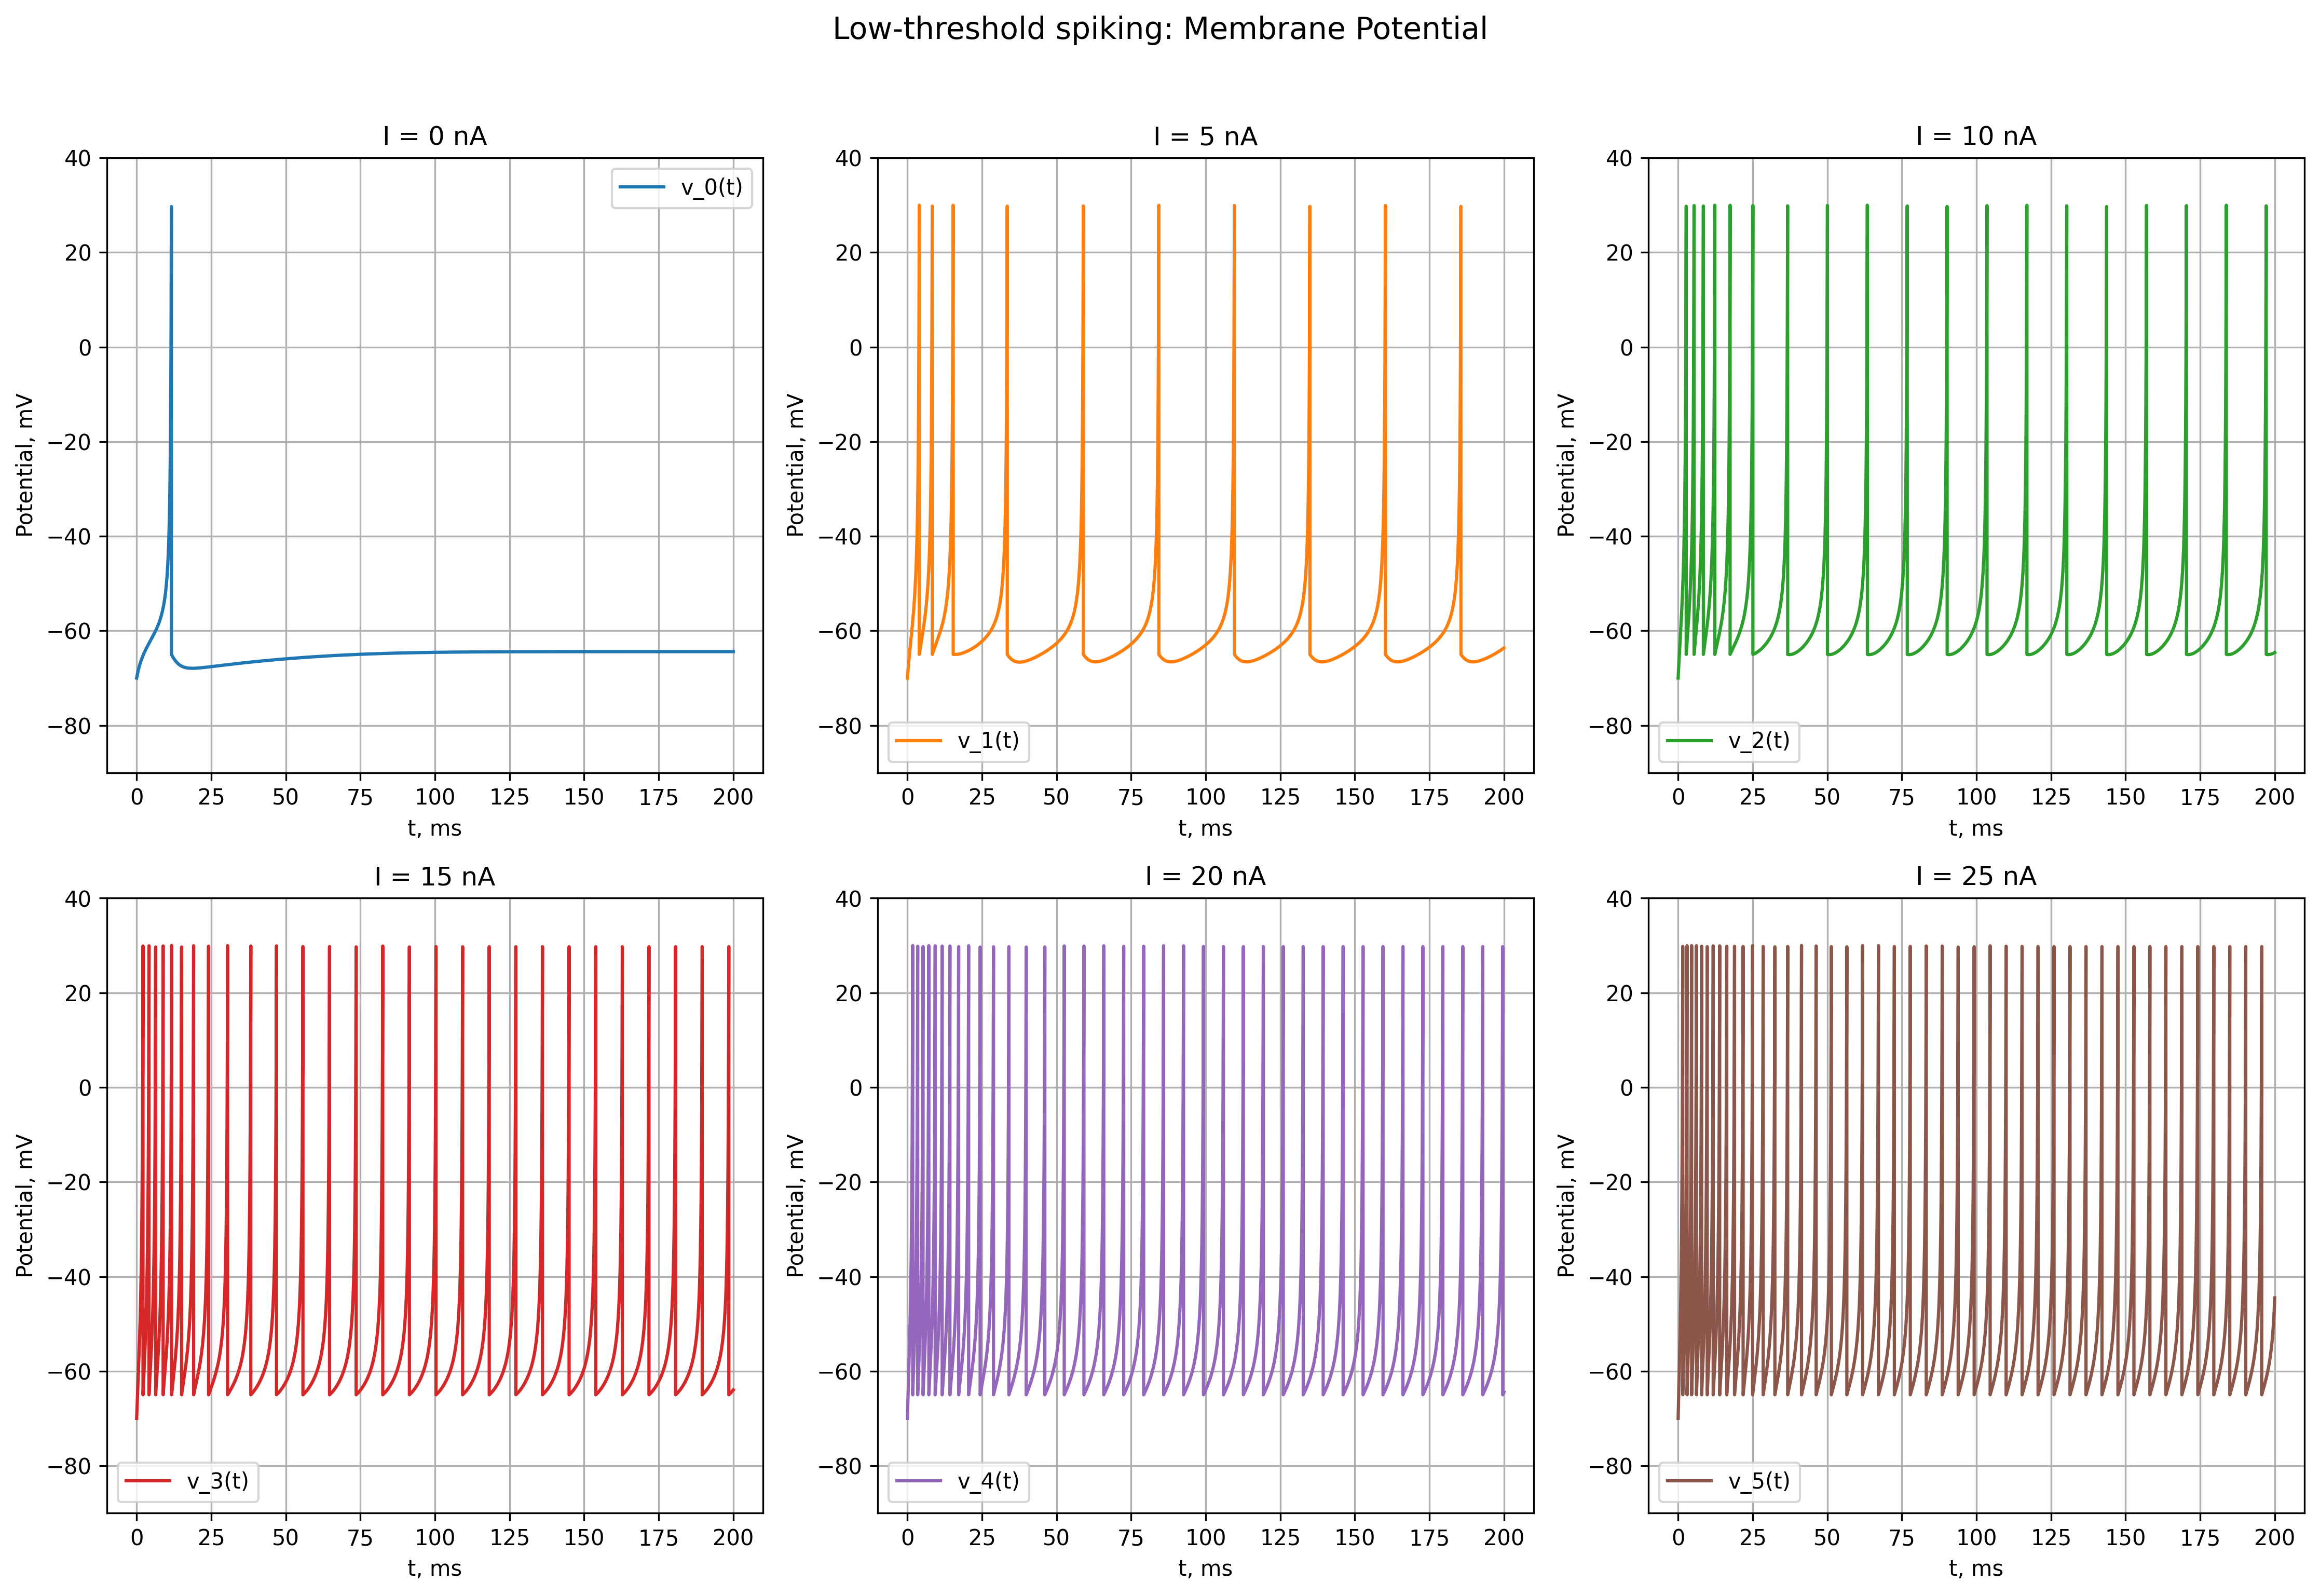
\includegraphics[width=1\linewidth]{pic/lts_different_I_potentials.png}}
	\caption{Графики $v(t)$ низкопорогового спайкового нейрона для разных значений $I$.}
	\label{lts_different_I_potentials}
\end{figure}

\begin{figure}[h]
	\center{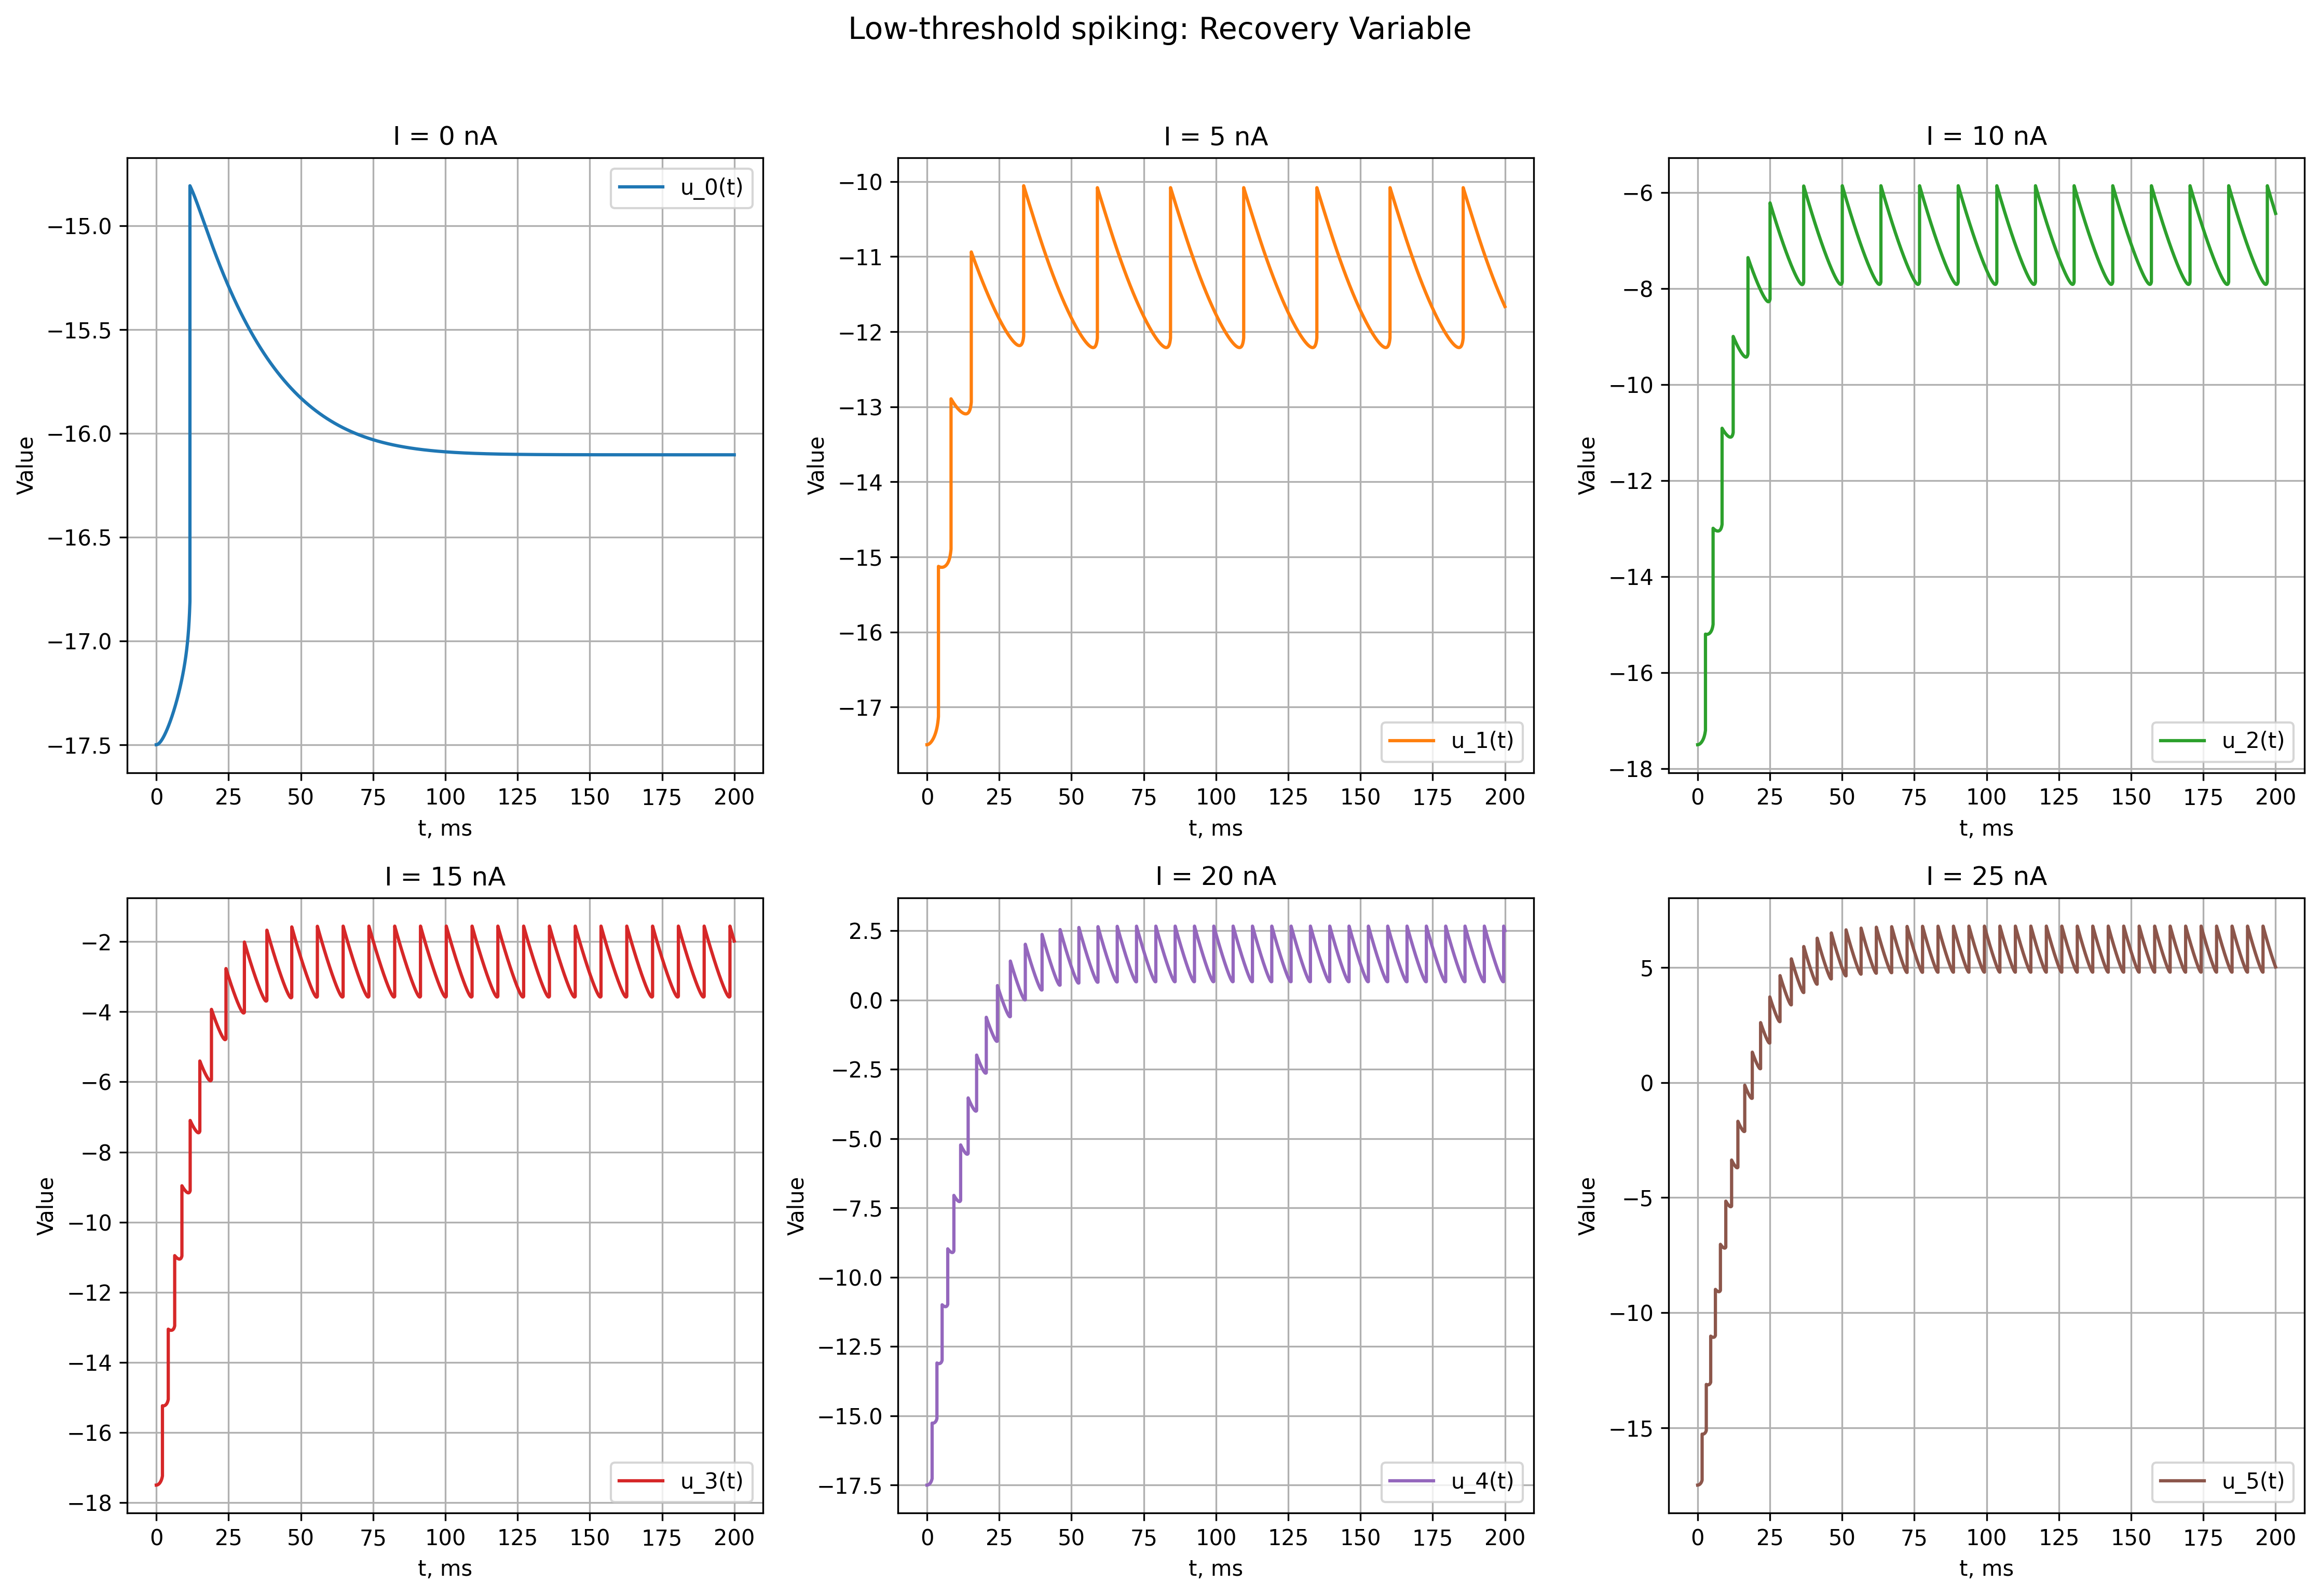
\includegraphics[width=1\linewidth]{pic/lts_different_I_recovery.png}}
	\caption{Графики $u(t)$ низкопорогового спайкового нейрона для разных значений $I$.}
	\label{lts_different_I_recovery}
\end{figure}

\begin{figure}[h]
	\center{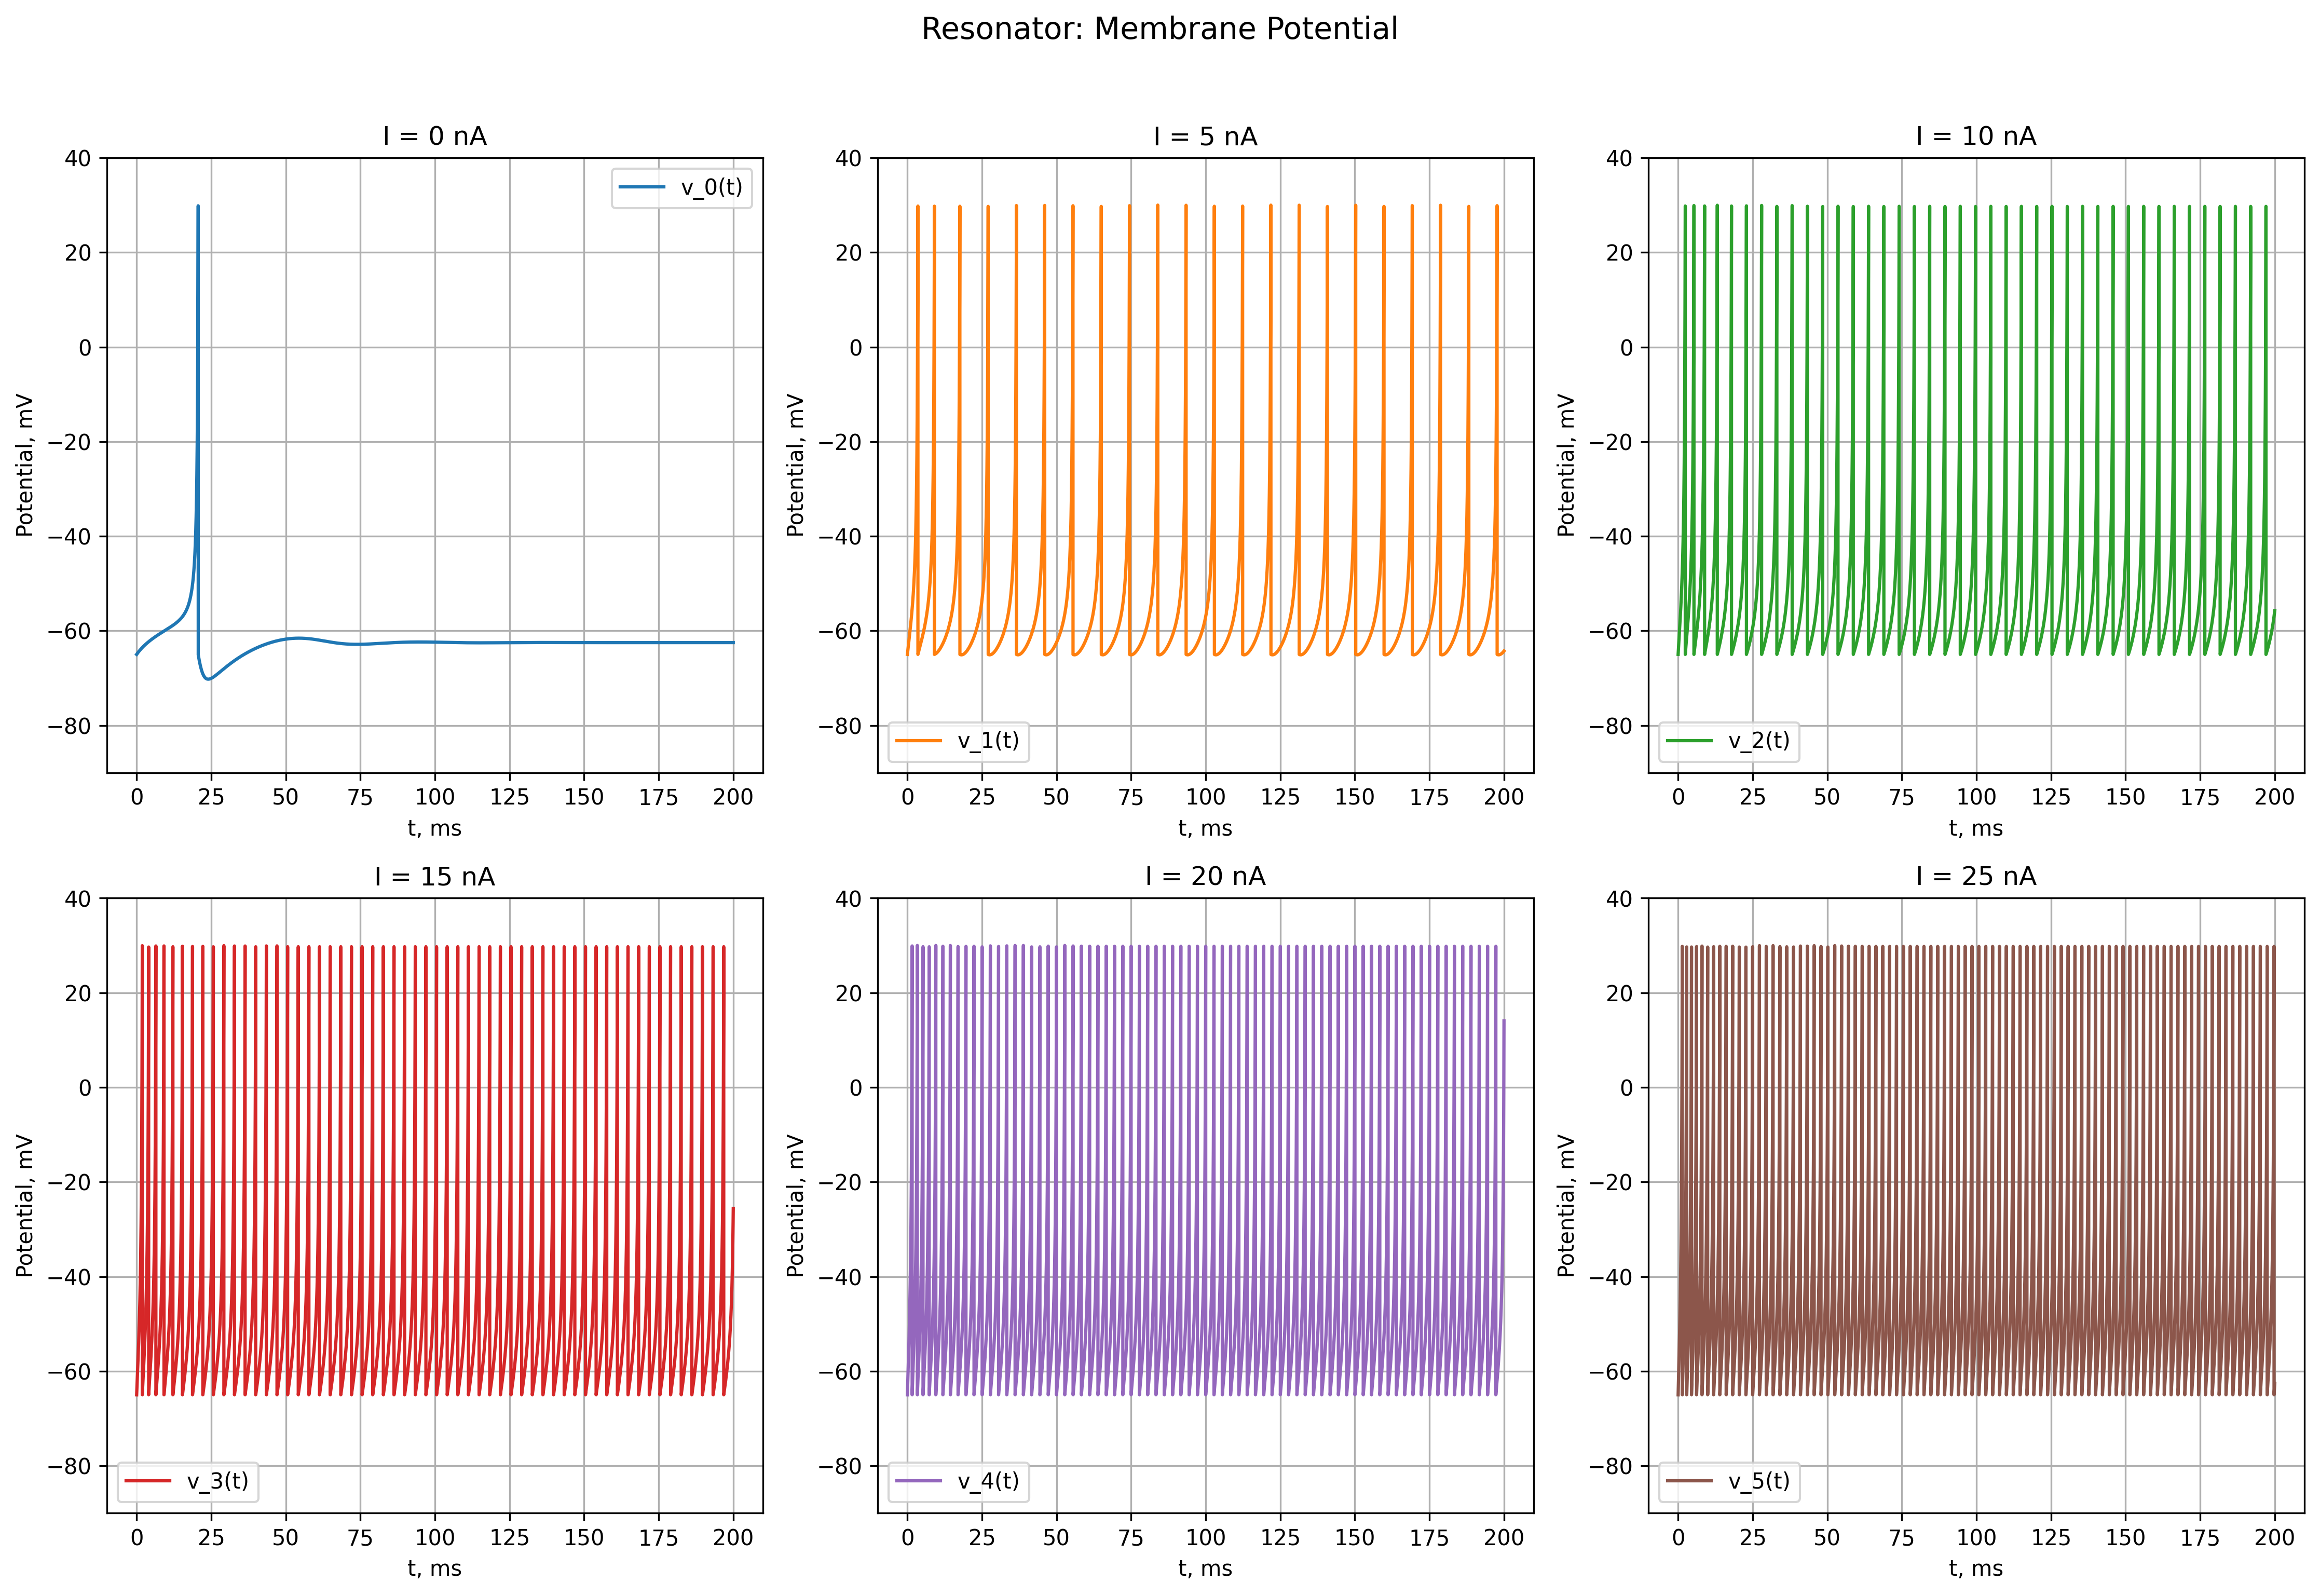
\includegraphics[width=1\linewidth]{pic/rz_different_I_potentials.png}}
	\caption{Графики $v(t)$ резонансного нейрона для разных значений $I$.}
	\label{rz_different_I_potentials}
\end{figure}

\begin{figure}[h]
	\center{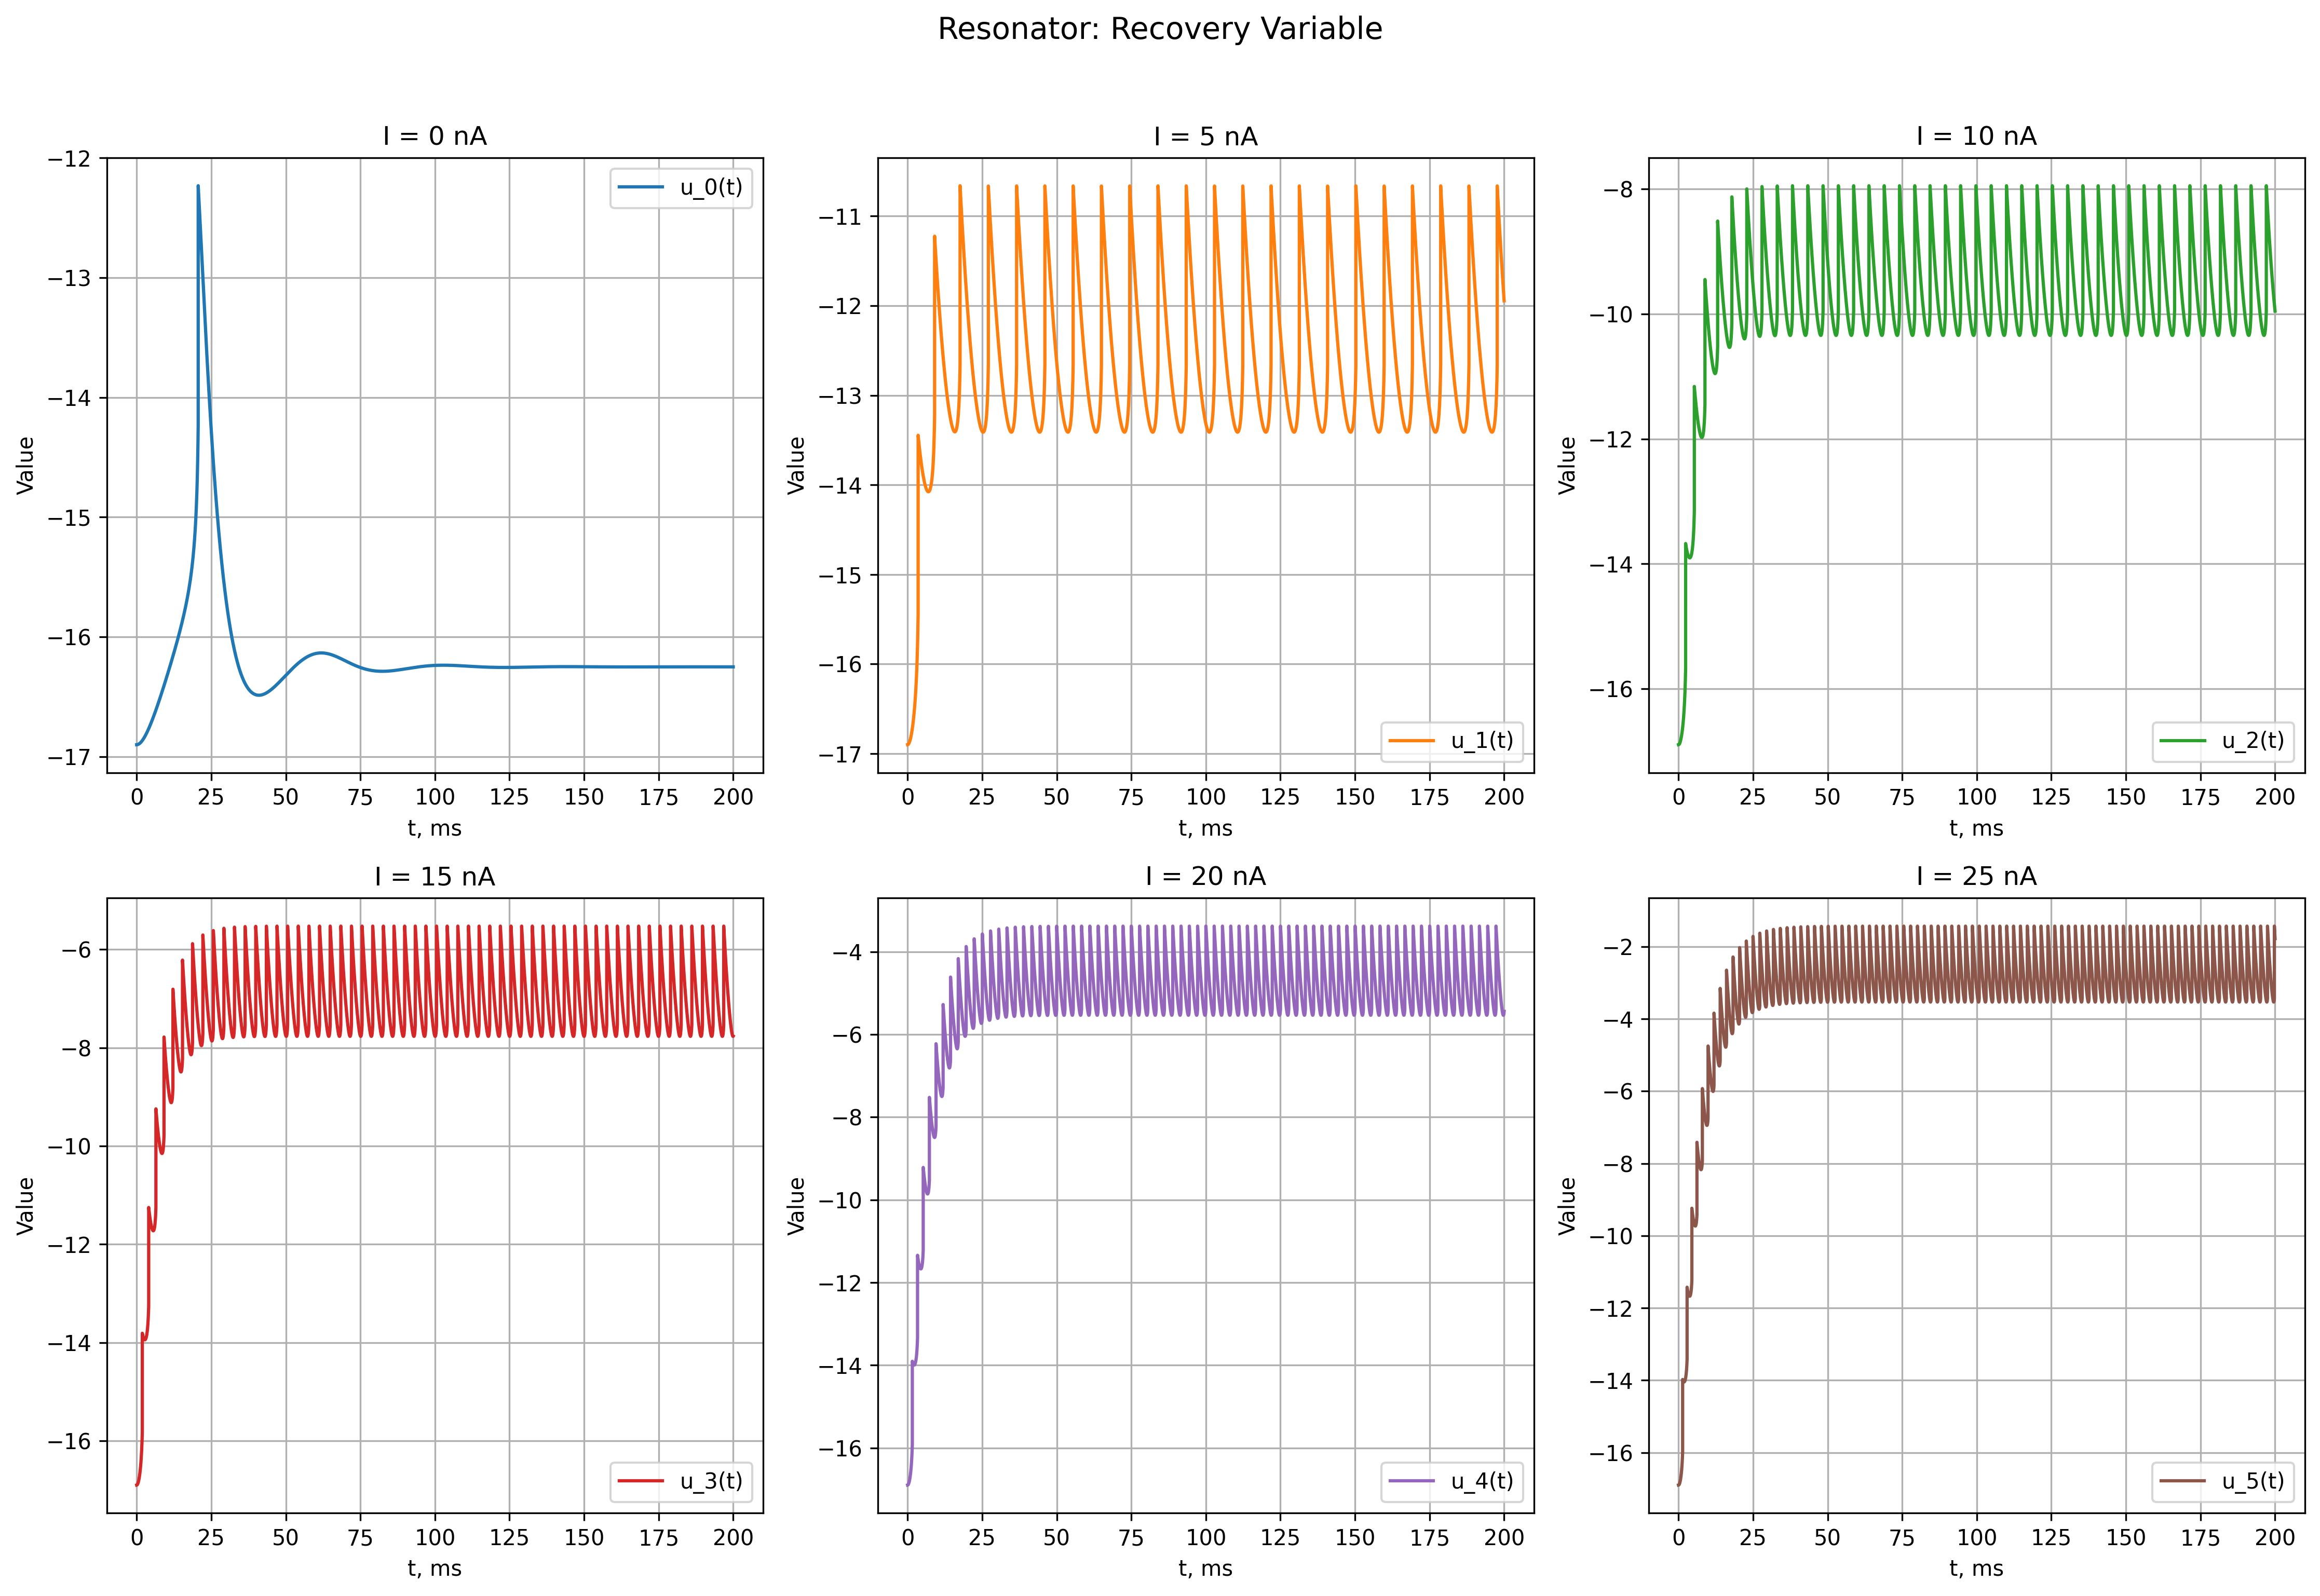
\includegraphics[width=1\linewidth]{pic/rz_different_I_recovery.png}}
	\caption{Графики $u(t)$ резонансного нейрона для разных значений $I$.}
	\label{rz_different_I_recovery}
\end{figure}

\begin{figure}[h]
	\center{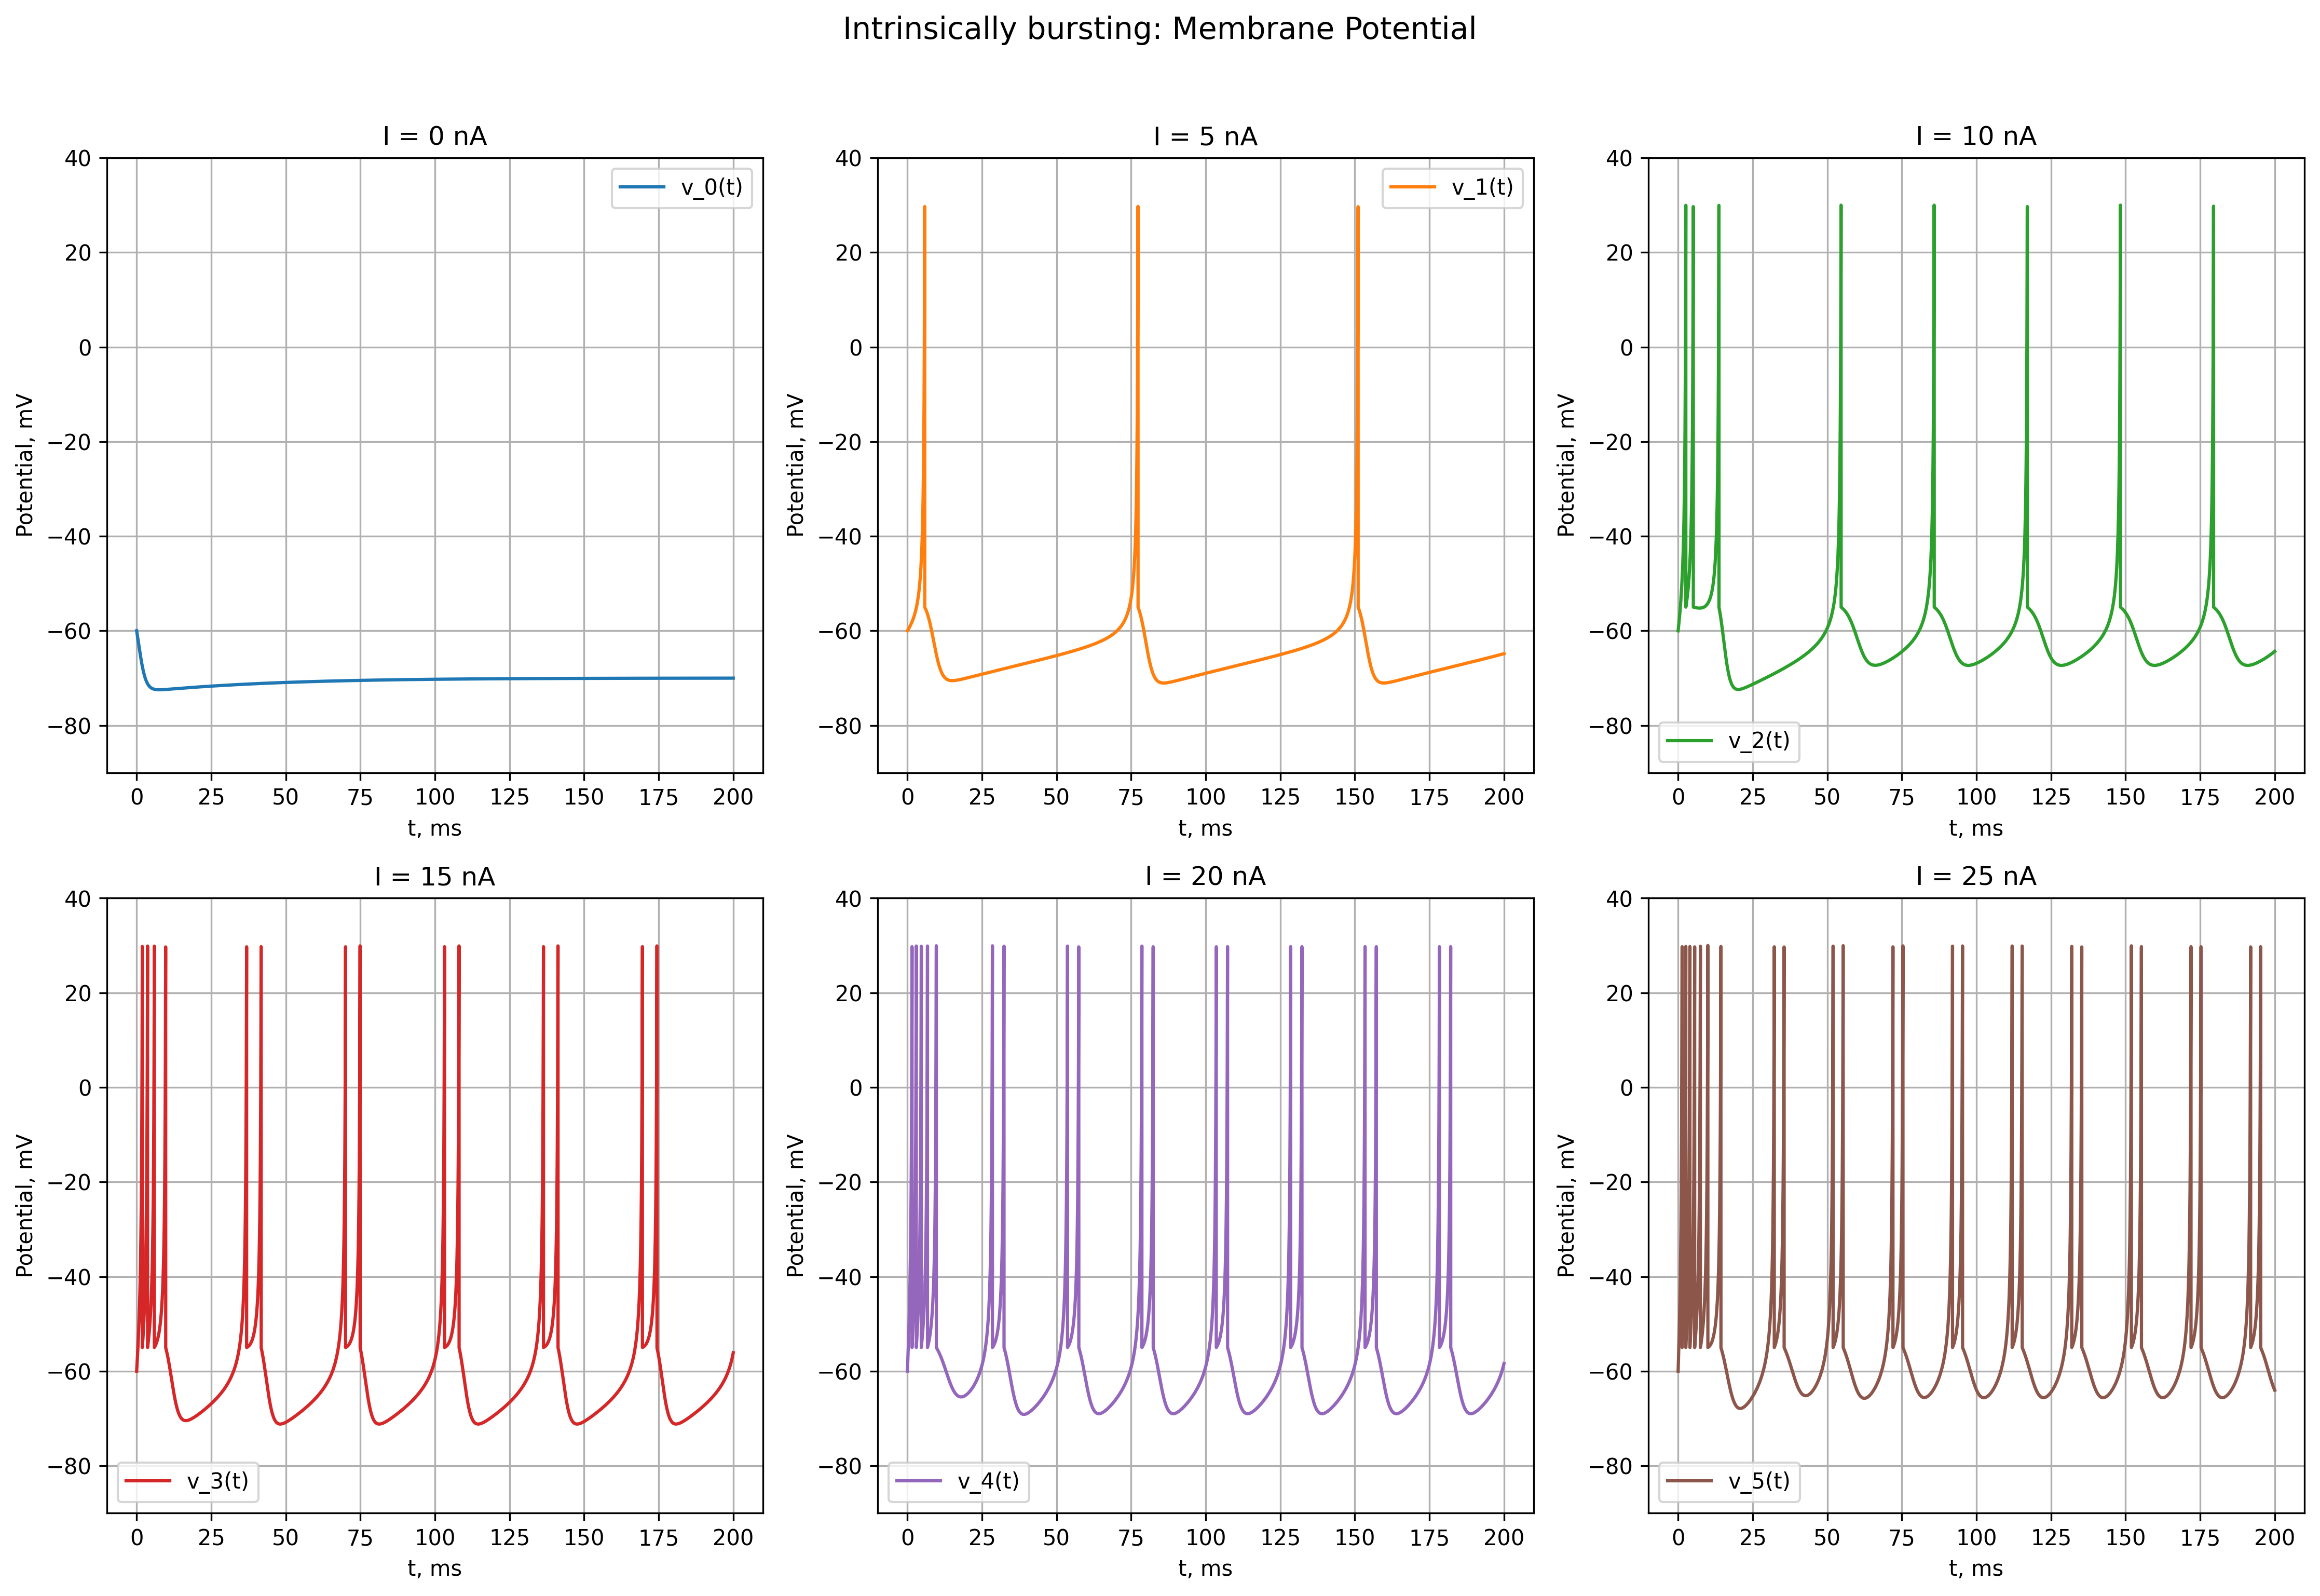
\includegraphics[width=1\linewidth]{pic/ib_different_I_potentials.png}}
	\caption{Графики $v(t)$ внутренне разрывного нейрона для разных значений $I$.}
	\label{ib_different_I_potentials}
\end{figure}

\begin{figure}[h]
	\center{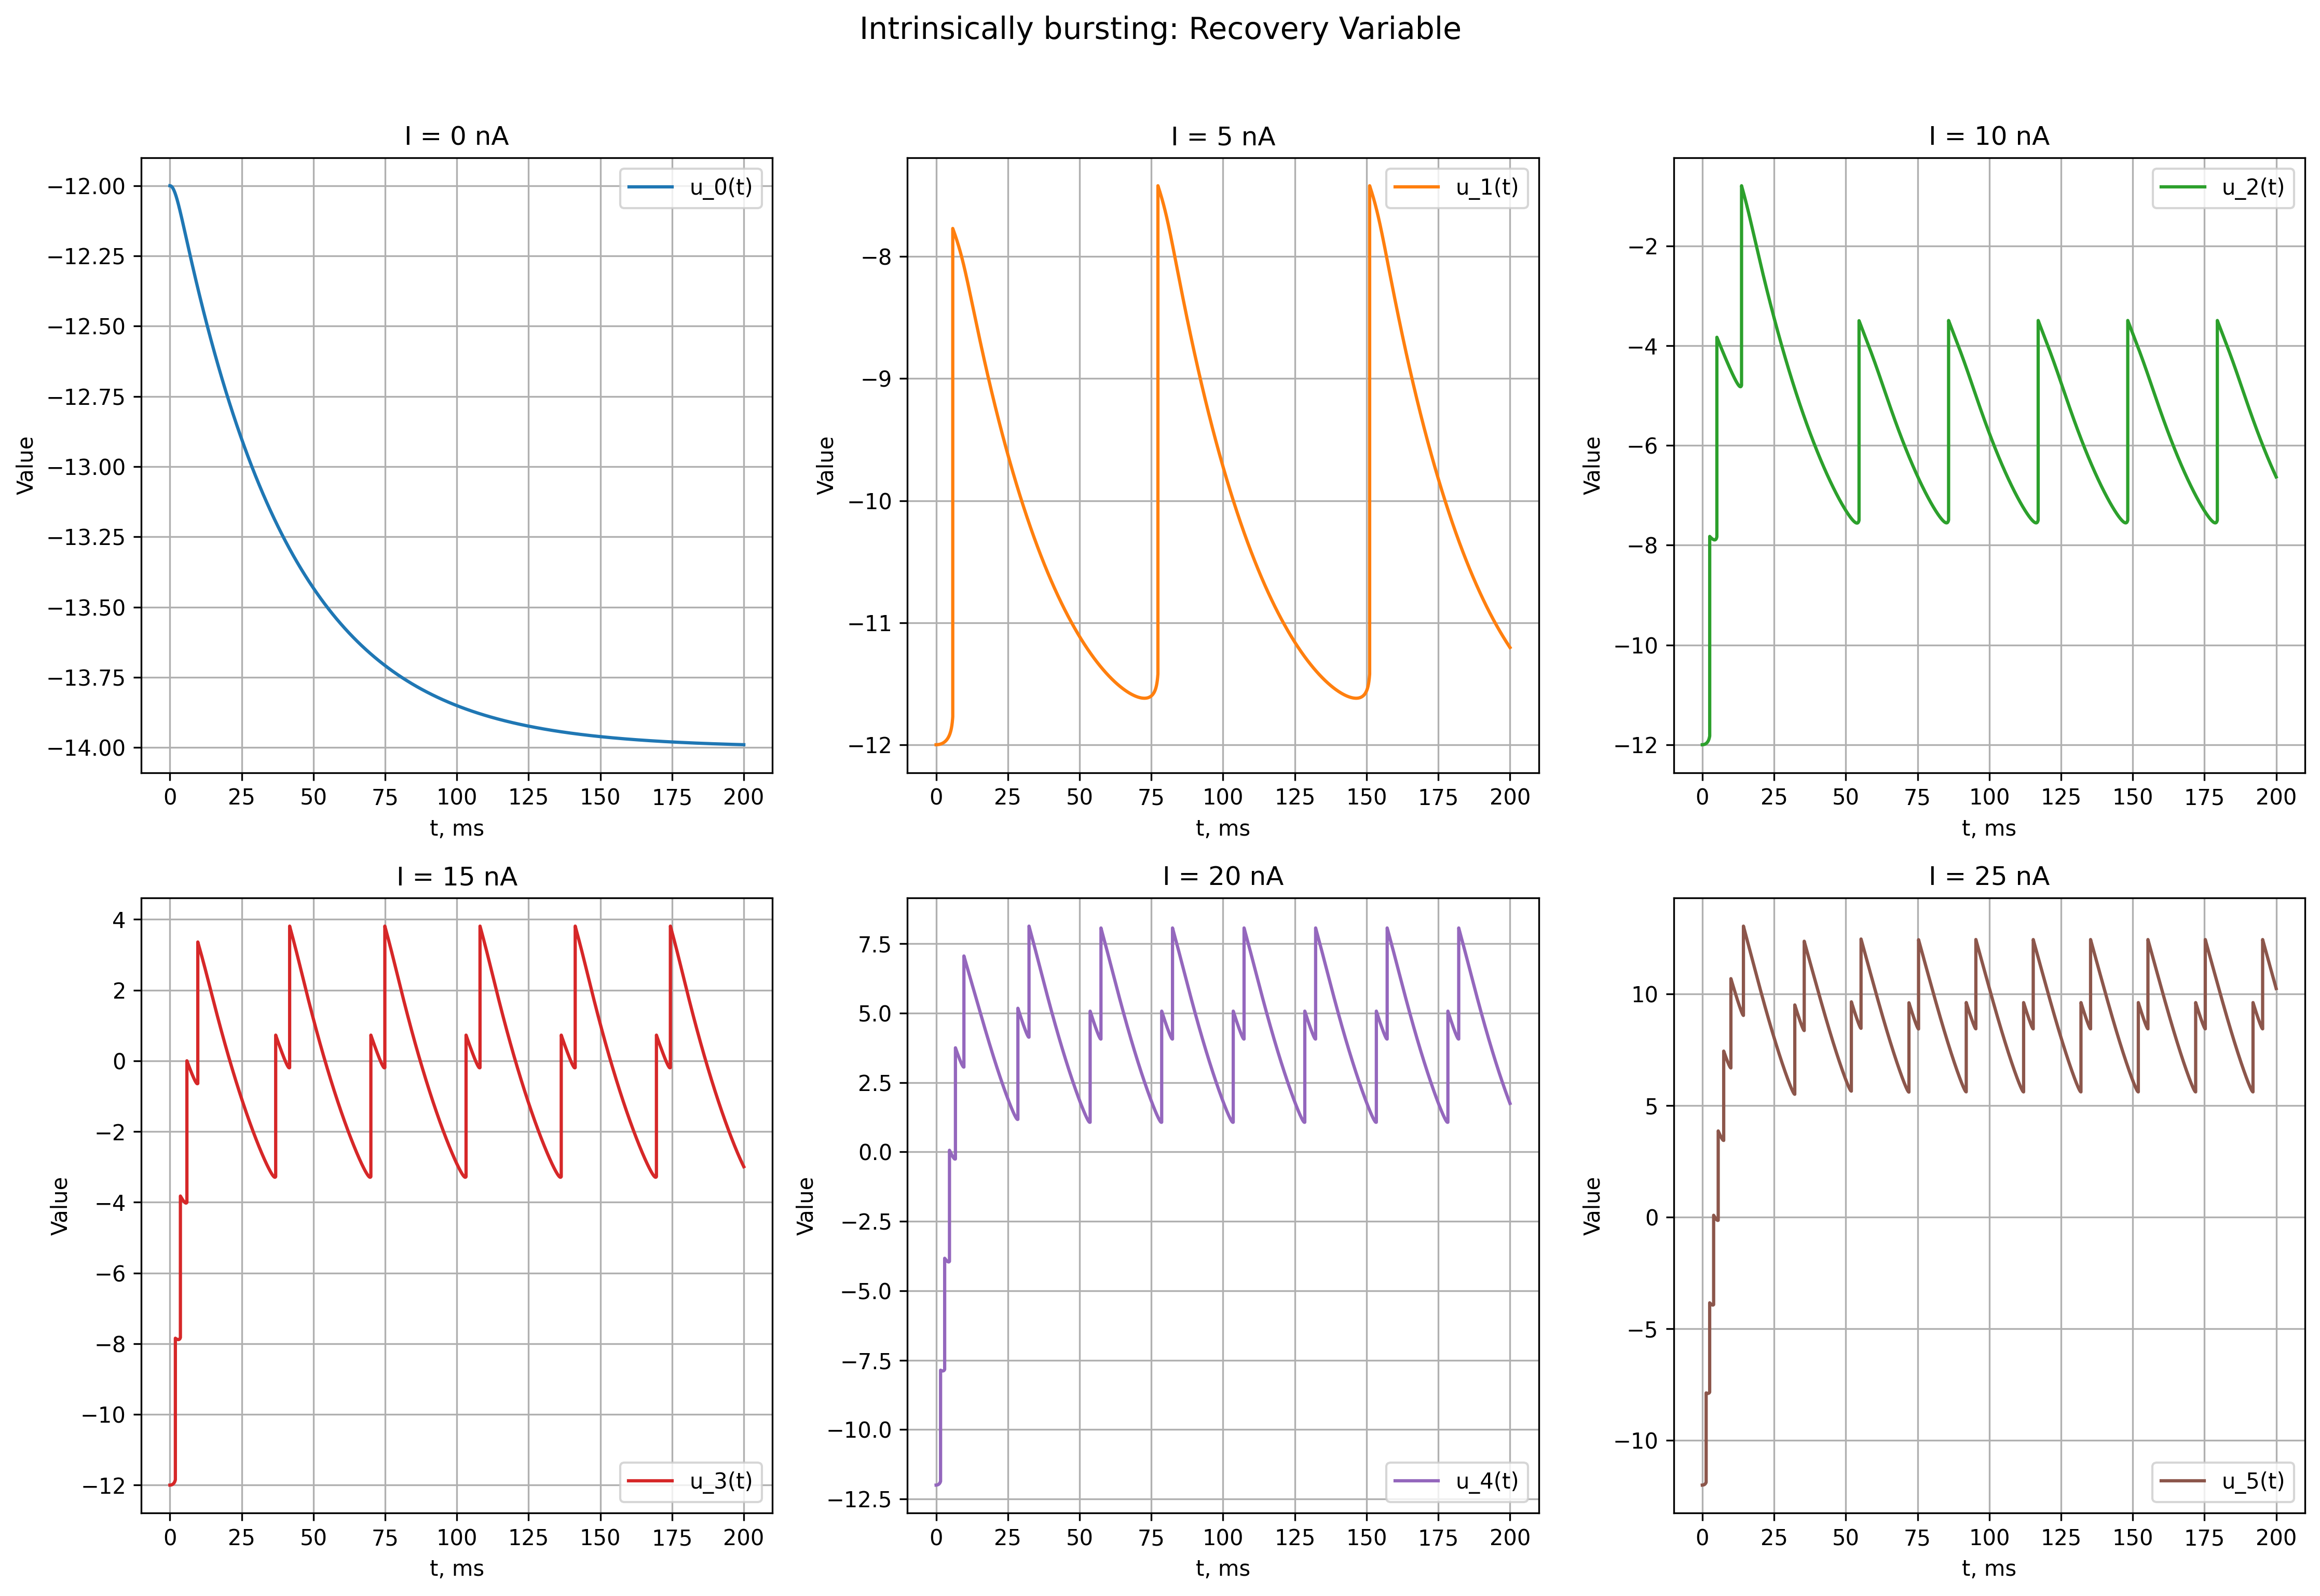
\includegraphics[width=1\linewidth]{pic/ib_different_I_recovery.png}}
	\caption{Графики $u(t)$ внутренне разрывного нейрона для разных значений $I$.}
	\label{ib_different_I_recovery}
\end{figure}

\begin{figure}[h]
	\center{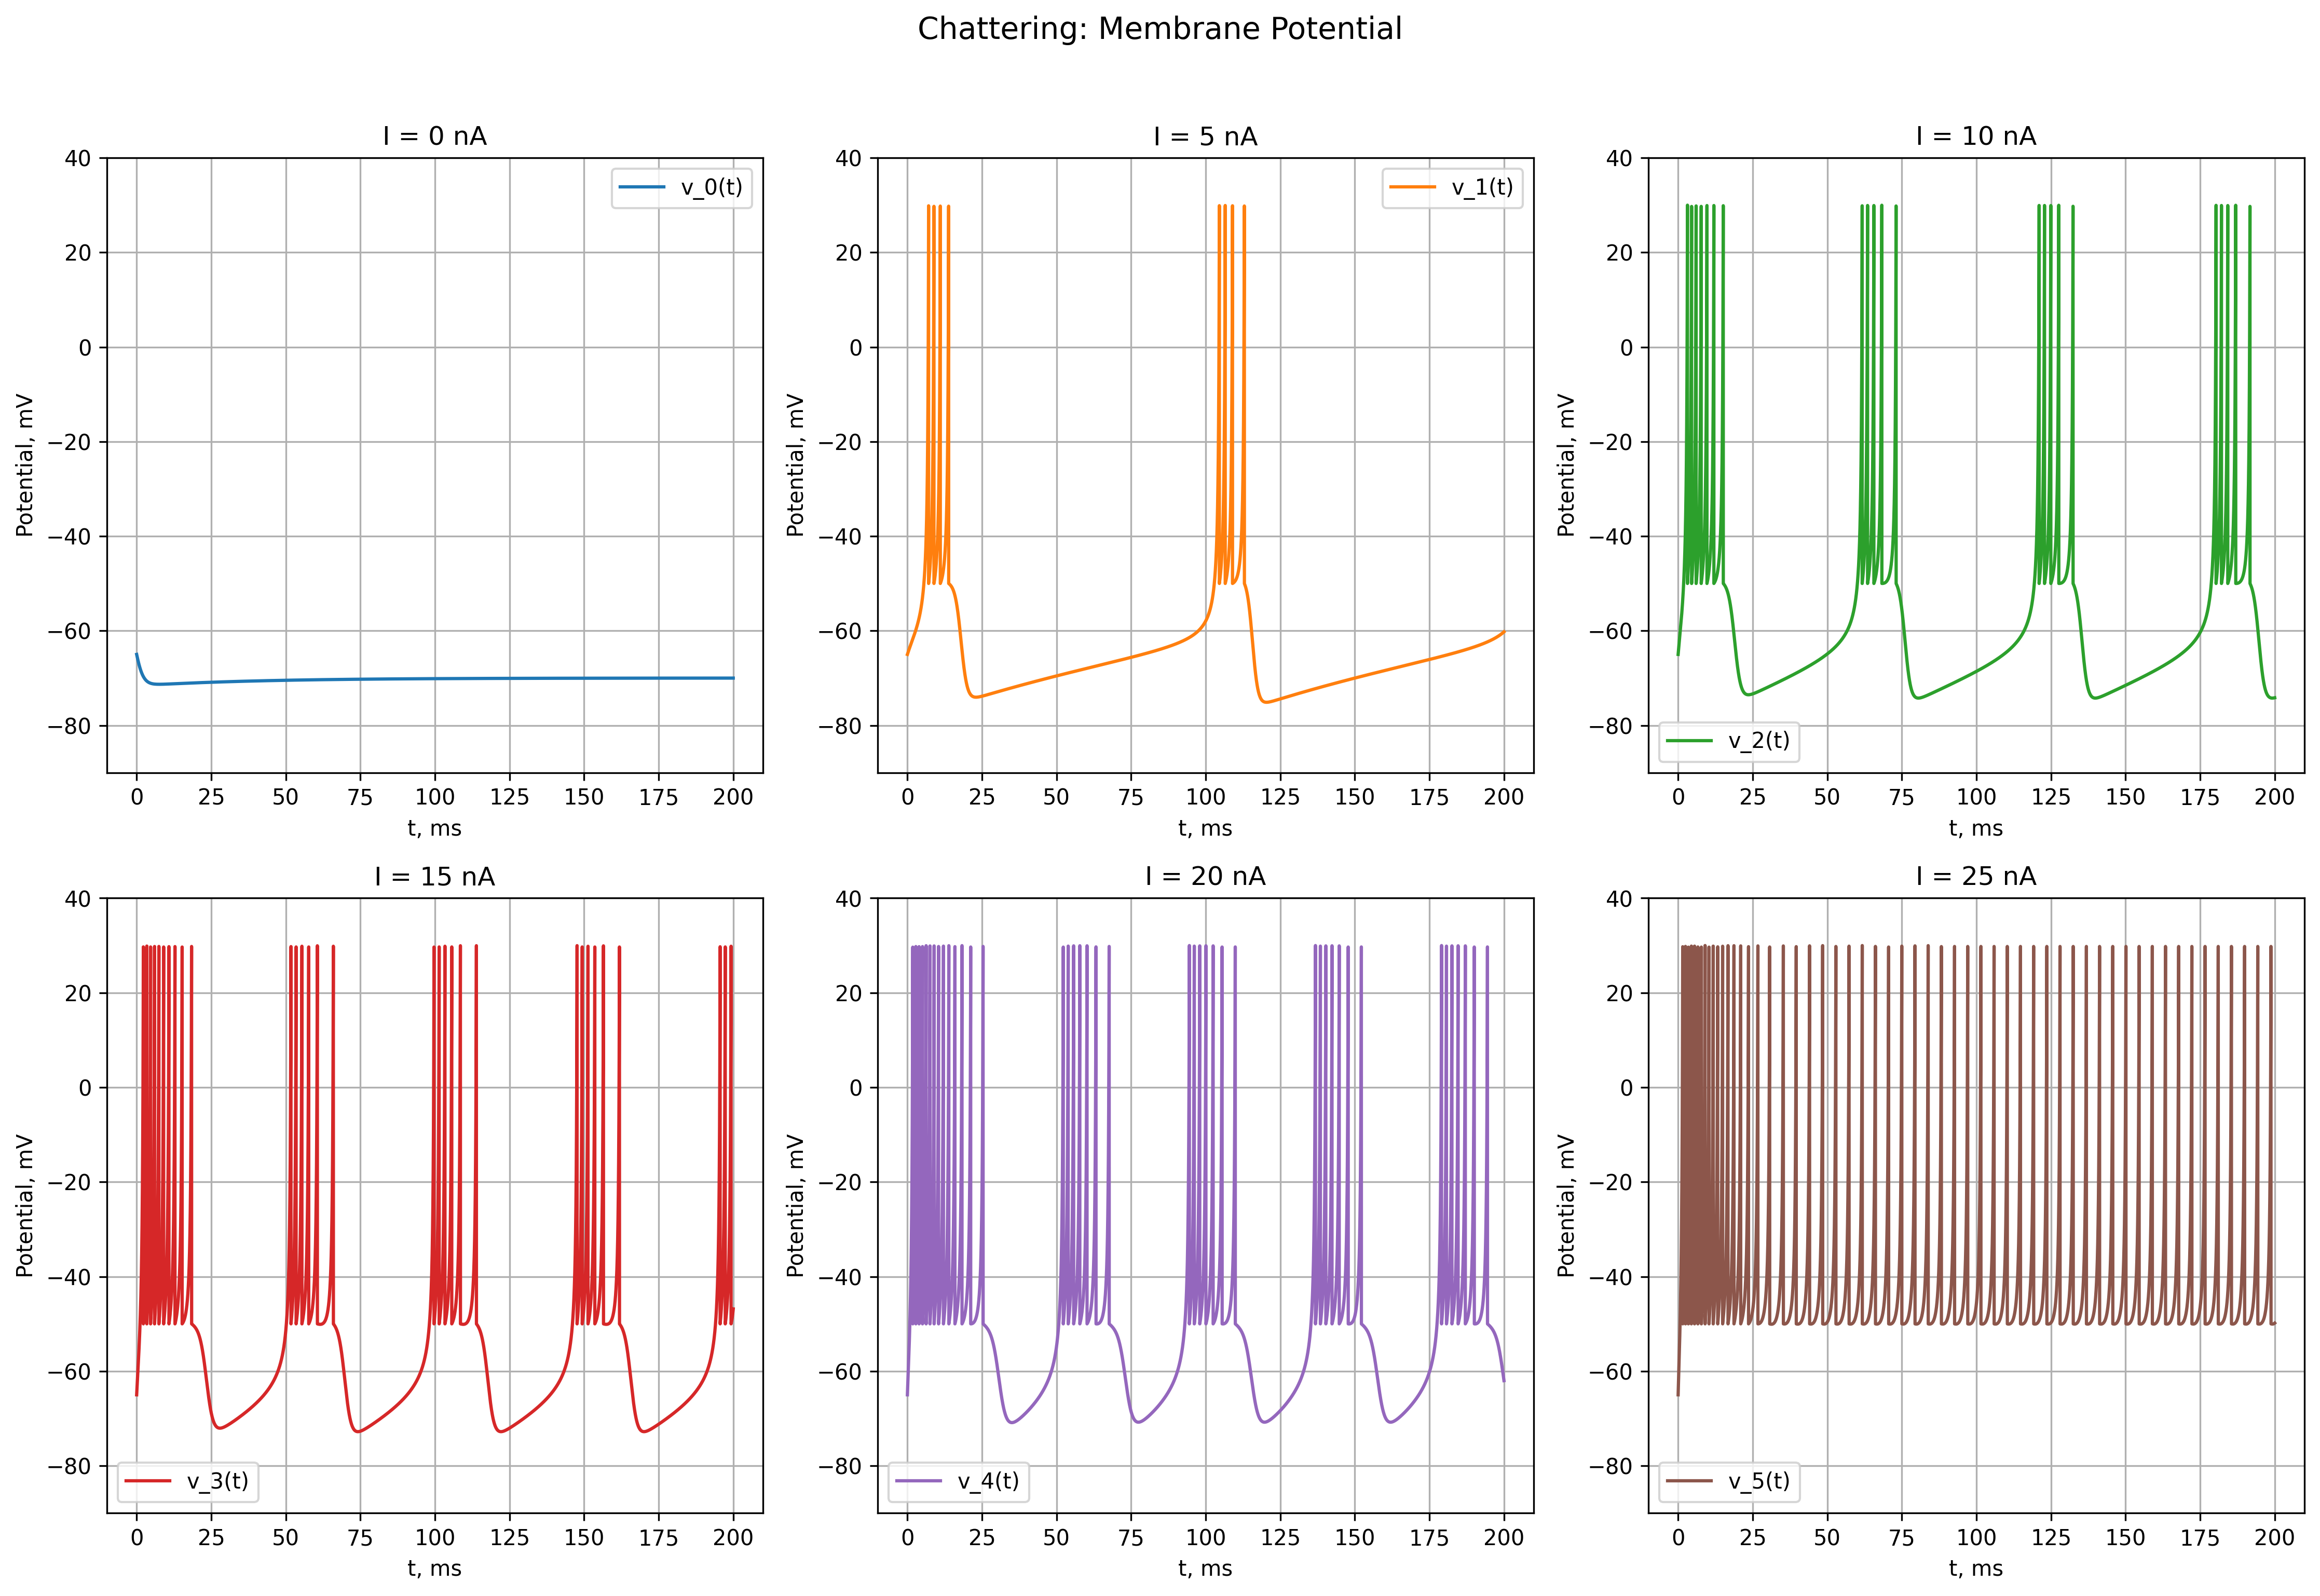
\includegraphics[width=1\linewidth]{pic/ch_different_I_potentials.png}}
	\caption{Графики $v(t)$ чаттерного нейрона для разных значений $I$.}
	\label{ch_different_I_potentials}
\end{figure}

\begin{figure}[h]
	\center{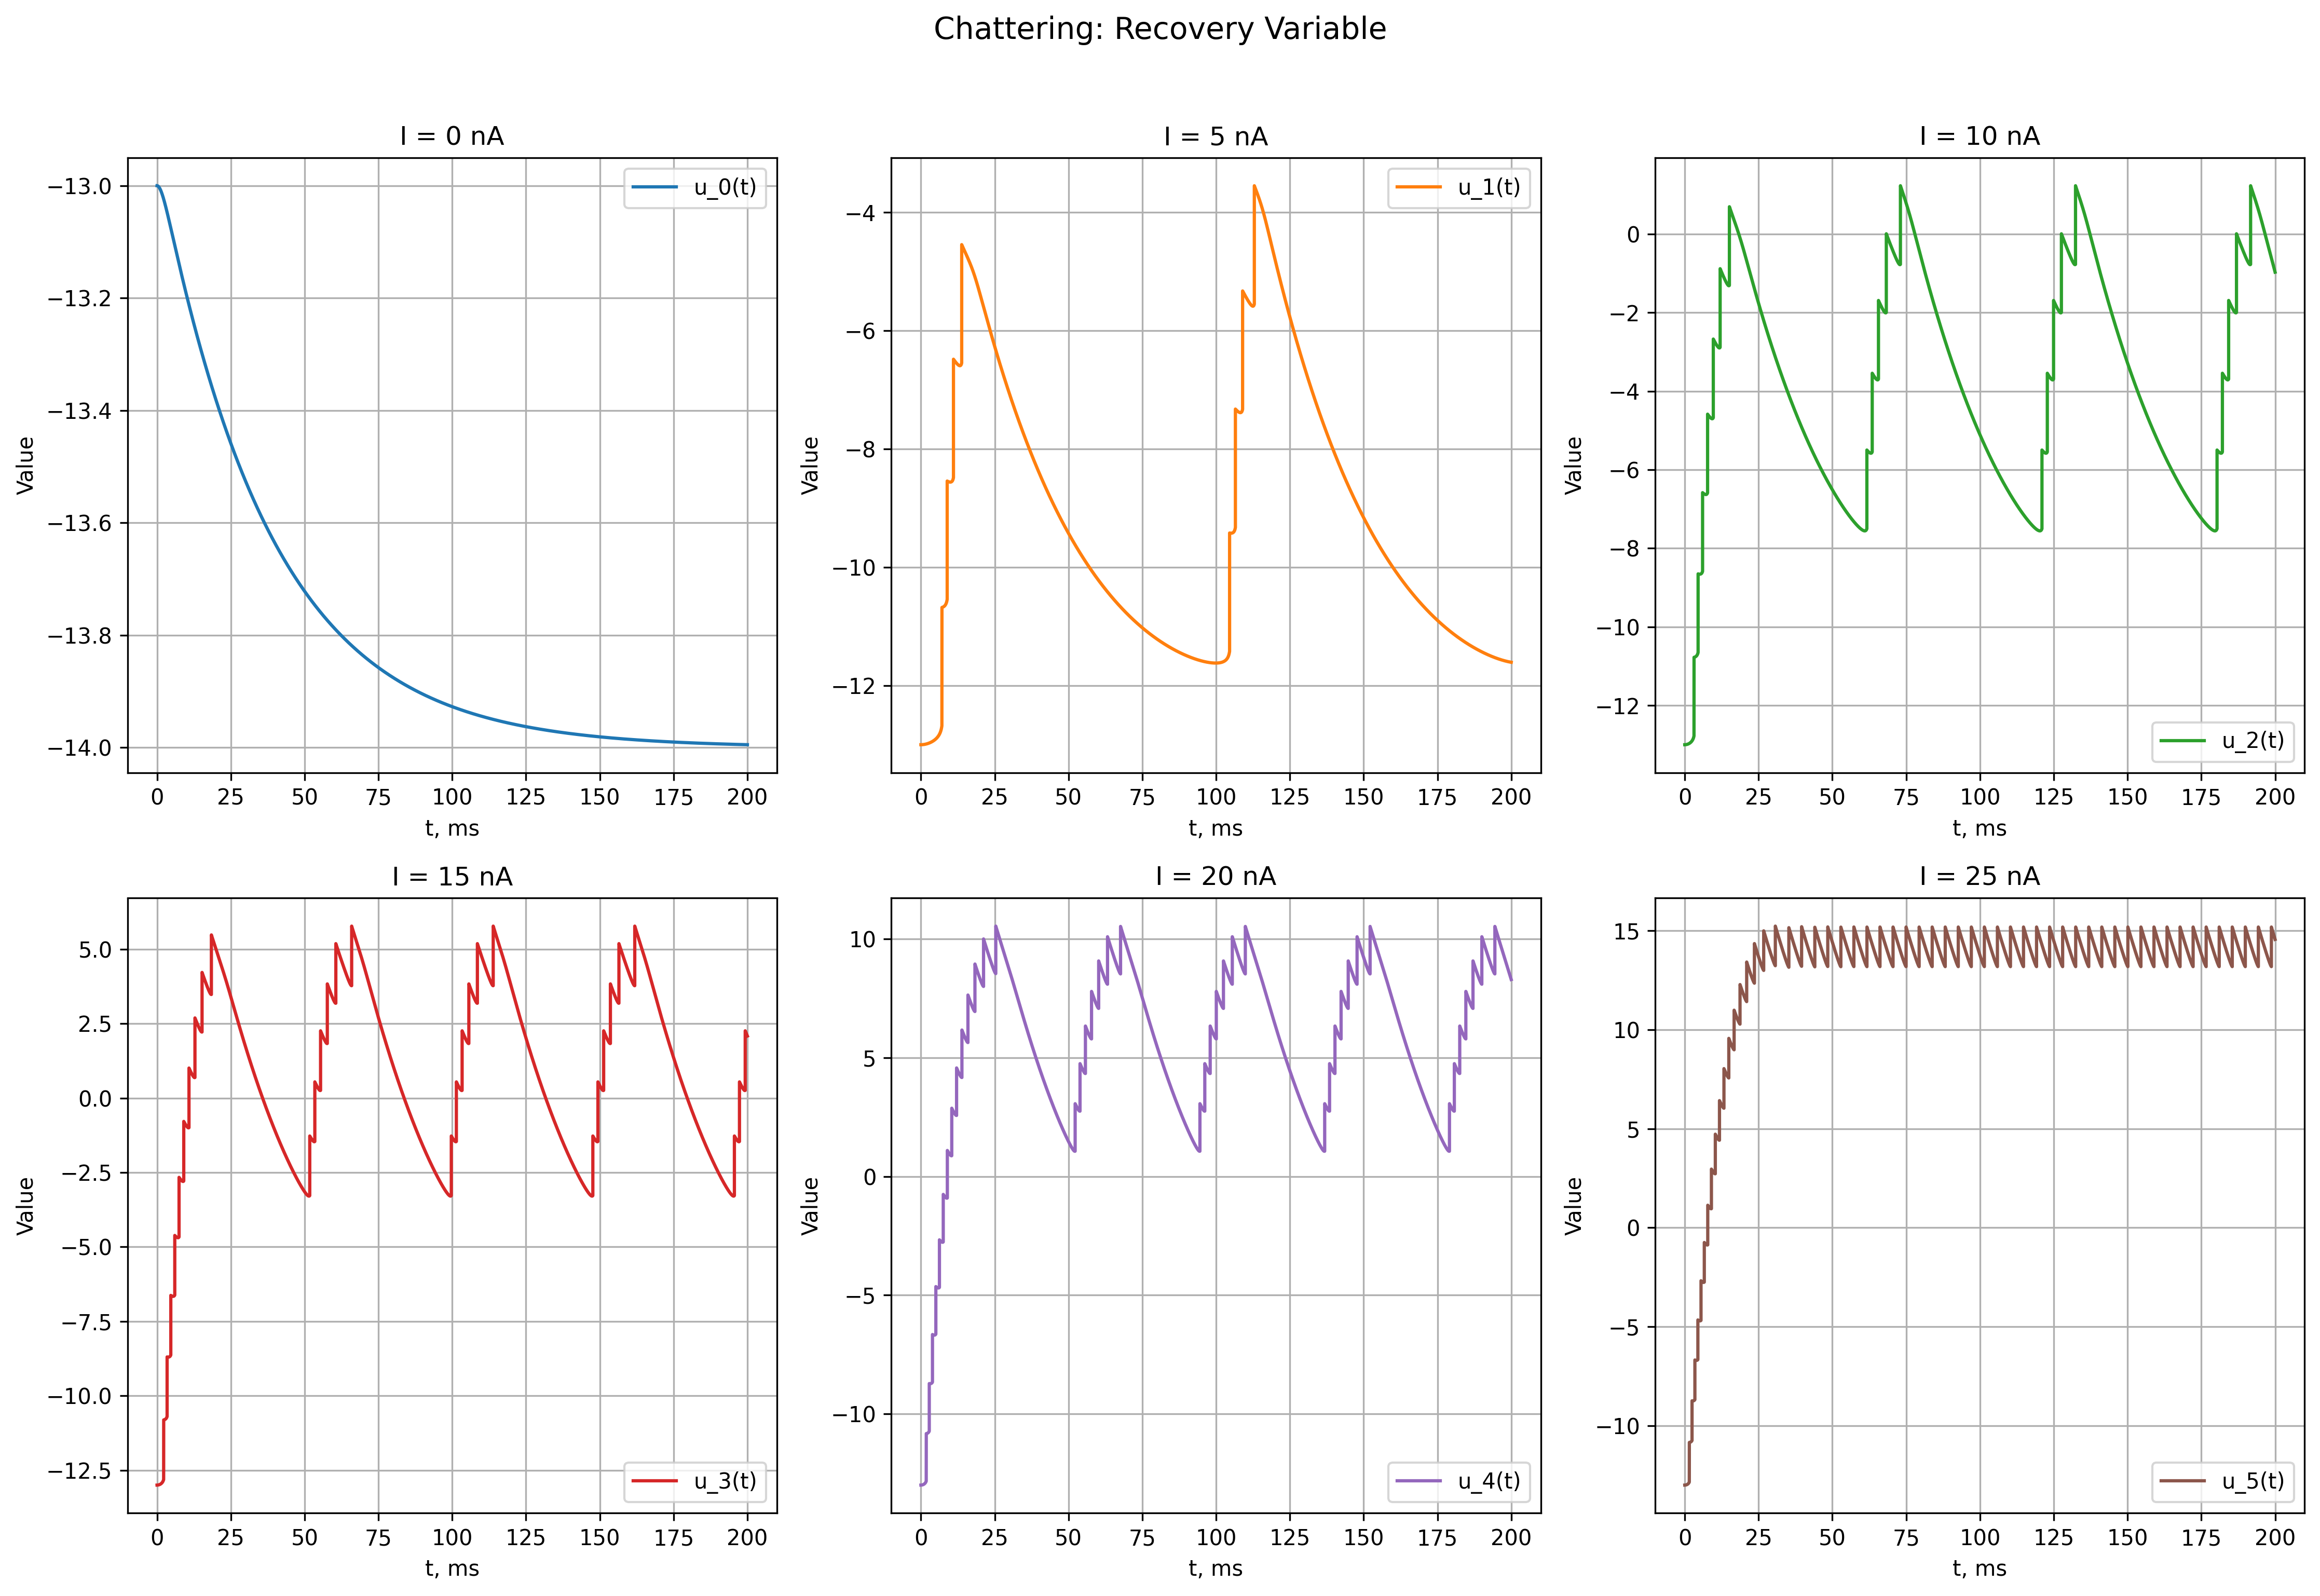
\includegraphics[width=1\linewidth]{pic/ch_different_I_recovery.png}}
	\caption{Графики $u(t)$ чаттерного нейрона для разных значений $I$.}
	\label{ch_different_I_recovery}
\end{figure}


\section{Анализ результатов}

В случае регулярно-спайкового нейрона наблюдаются спайки с интервалом, который увеличивается с течением времени (рисунок \ref{1_rs}). Для быстро-спайкового нейрона характерна постоянная высокая частота возникновения спаек (рисунок \ref{1_fs}), особенно разница заметна при сравнении с регулярно-спайковым нейроном. В результате моделирования низкопорогового нейрона отчетливо видно постепенное снижение частоты спаек, в начале наблюдаются высокочастотные спайки (рисунок \ref{1_lts}). Моделирование резонансного нейрона демонстрирует небольшое повышение частоты спаек в начале с последующим увеличением интервала между спайками (рисунок \ref{1_rz}). Визуализация динамики внутренне разрывного нейрона показывает, что частота спаек в начале выше, а дальше образуется высокачастотные участки спаек с относительно большими интервалами между ними (рисунок \ref{1_ib}). Для чаттерного нейрона характерно образование высокочастотных участков спаек с интервалом между ними (рисунок \ref{1_ch}).

Выполненное моделирование подтверждает характеристики динамики нейрона Ижикевича с определенными наборами параметров, описанными в предыдущей главе.

Повышение значений тока $I$ для всех рассмотренных моделей приводит к росту частоты спаек (рисунки \ref{rs_different_I_potentials}-\ref{ch_different_I_recovery}), а в случае чаттерного нейрона еще и к стиранию интервала между высокочастотными участками спаек.

\section{Листинг кода}

\inputminted[
breakanywhere=true, 
breaklines=true,
breaksymbolleft=\small\carriagereturn, 
frame=lines,
linenos,
fontsize=\footnotesize,
baselinestretch=0.8
]{python}{big_file.py}
\captiontextt{Листинг 1 --- Исходный код программы для моделирования динамики отдельных нейронов.}





\endinput